
\documentclass[english,a4paper]{article}



\usepackage{ifdraft}
\usepackage{pgf}
\usepackage{xspace}


\usepackage[english]{babel}
\usepackage{geometry}
\usepackage{makeidx}
\usepackage{tabto}
\usepackage{fancyhdr}
\usepackage{multicol}


\usepackage{marvosym}
\usepackage{amsfonts}
\usepackage{amssymb}
\usepackage{stmaryrd}
\usepackage{braket}
\usepackage{bbold}
\usepackage{bbm}

\usepackage{braket}
\usepackage{extarrows}
\usepackage{colonequals}


\usepackage{mathtools}
\usepackage{amsmath}
\usepackage{amsthm}
\usepackage{cases}
\usepackage{multirow, bigdelim}
\usepackage{nicefrac}
\usepackage{relsize}


\usepackage{algorithm}
\usepackage{algorithmic}


\usepackage{array}
\usepackage{enumerate}
\usepackage[inline]{enumitem}
\usepackage{graphicx}
\usepackage{caption}
\usepackage{subcaption}
\usepackage{tikz}
\usepackage{tkz-graph}
\usepackage{float}
\usepackage{pdfpages}
\usepackage[nopgf,nographicx,nobookmark]{incgraph}
\usepackage{longtable}
\usepackage{array}
\usepackage{multirow}
\usepackage{scrextend,rotating}
\usepackage{makecell}


\usepackage{hyperref}


\usepackage{tocbasic}
\usepackage{cite}
\usepackage{url}


\usepackage{xcolor,color, colortbl}


\usepackage{marginnote} \usepackage[colorinlistoftodos]{todonotes}
\usepackage{textcomp}




\allowdisplaybreaks[1]
\graphicspath{ {images/} }



\setcounter{tocdepth}{1}
\newcommand{\emptypage}{\newpage\null\thispagestyle{empty}\newpage}



\newcommand{\todoinline}[1]{\todo[inline, caption = {}]{#1}}




\usetikzlibrary{fit}
\usetikzlibrary{arrows}
\usetikzlibrary{petri}
\usetikzlibrary{topaths}
\usetikzlibrary{positioning}
\usetikzlibrary{patterns}
\usetikzlibrary{decorations.pathreplacing}
\usetikzlibrary{calc}
\usetikzlibrary{shapes}
\usetikzlibrary{trees}
\usetikzlibrary{intersections}
\tikzset{>=latex'}



\theoremstyle{plain}
\newtheorem{theorem}             {Theorem}[section]
\newtheorem{lemma}      [theorem]{Lemma}
\newtheorem{corollary}  [theorem]{Corollary}
\newtheorem{proposition}[theorem]{Proposition}
\newtheorem{claim}      [theorem]{Claim}
\newtheorem{conjecture} [theorem]{Conjecture}
\newtheorem{assumption} [theorem]{Assumption}

\theoremstyle{definition}
\newtheorem{definition} [theorem]{Definition}
\newtheorem{problem}	[theorem]{Problem}
\newtheorem{example}    [theorem]{Example}
\newtheorem{remark}     [theorem]{Remark}
\newtheorem{observation}[theorem]{Observation}





\newcommand{\Nat}{\ensuremath{\mathbb{N}}}
\newcommand{\Rel}{\ensuremath{\mathbb{R}}}


\DeclareMathOperator{\bd}{bd}
\DeclareMathOperator{\id}{id}
\DeclareMathOperator{\argmin}{argmin}
\DeclareMathOperator{\argmax}{argmax}
\DeclareMathOperator{\rank}{rank}

\DeclareMathOperator{\dist}{dist}
\DeclareMathOperator{\Aut}{Aut}


\newcommand{\norm}[1]{\left\lVert#1\right\rVert}
\newcommand{\scal}[1]{\left\langle #1 \right\rangle}
\newcommand{\absAdaptable}[1]{\left| #1 \right|}
\newcommand{\abs}[1]{| #1 |}
\newcommand{\compl}[1]{\ensuremath{\overline{#1}}}
\DeclareMathOperator{\lcm}{lcm}
\newcommand{\reverseFunction}[1]{\ensuremath{#1^{-1}}}

\newcommand{\restr}[2]{
	\ensuremath{
		\left.\kern-\nulldelimiterspace
		#1
		\vphantom{\big|}
		\right|_{#2}
	}
}

\newcommand{\disjointUnion}{\ensuremath{\mathbin{\dot{\cup}}}}
\newcommand{\srg}[1]{srg\left(#1\right)}

\newcommand{\calO}[1]{\ensuremath{\mathcal{O}(#1)}}
\newcommand{\reducesMOto}[1]{\leqslant^{#1}_{\lang{mo}}}
\newcommand{\reducesTMto}[1]{\leqslant^{#1}_{\lang{TM}}}







 




\title{
	An Upper Bound on the Weisfeiler-Leman Dimension\footnote{The research leading to these results has received funding from the European Research Council (ERC) under the European Union’s Horizon 2020 research and innovation programme (EngageS: grant agreement No.\ 820148).}
}
\author{
	Thomas Schneider and Pascal Schweitzer\\
	TU Darmstadt
}



\definecolor{darkgreen}{rgb}{0,0.6,0}
\definecolor{darkred}{RGB}{128, 0, 0}
\definecolor{darkblue}{RGB}{51, 204, 204}
\definecolor{darkyellow}{RGB}{204,204,0}
\definecolor{fuchsia}{RGB}{255,0,255}

\definecolor{lightblue}{RGB}{173,216,230}
\definecolor{lightred}{RGB}{233,150,122}
\definecolor{lightyellow}{RGB}{250,250,210}
\definecolor{lightgray}{RGB}{198,198,198}





\hypersetup{breaklinks=true}
\urlstyle{same}
\Urlmuskip=0mu plus 1mu\relax
\bibliographystyle{alpha}

\definecolor{hrefblue}{rgb}{0.5,0.5,1.0}
\definecolor{hrefred}{rgb}{0.5,0,0}
\definecolor{hrefgreen}{rgb}{0,0.5,0}
\definecolor{hrefblue}{rgb}{0,0,0.5}

\hypersetup{colorlinks,linkcolor=hrefred,filecolor=hrefgreen,urlcolor=hrefred,citecolor=hrefblue}

\definecolor{labelkey}{RGB}{51, 204, 204}




\def\env@matrix{\hskip -\arraycolsep
	\let\@ifnextchar\new@ifnextchar
	\array{*\c@MaxMatrixCols c}}

\makeatletter
\renewcommand*\env@matrix[1][c]{\hskip -\arraycolsep
	\let\@ifnextchar\new@ifnextchar
	\array{*\c@MaxMatrixCols #1}}
\makeatother




\setlist[enumerate]{label=(\arabic*)}
 


\DeclareMathOperator{\Fibers}{F}
\newcommand{\coherentConfig}{\ensuremath{\mathfrak{X}}}
\newcommand{\fibers}[1]{\ensuremath{\Fibers \left( #1 \right)}}
\newcommand{\interspace}[2]{\ensuremath{\coherentConfig[#1,#2]}}
\newcommand{\inducedCC}[1]{\ensuremath{\coherentConfig[#1]}}
\newcommand{\intDegree}[1]{\ensuremath{\Deg \left( #1 \right)}}
\newcommand{\minimalDegree}[2]{\Deg(#1,#2)}
\DeclareMathOperator*{\ul}{ul}

\DeclareMathOperator*{\Type}{T}
\newcommand{\type}[1]{\ensuremath{\Type\left(#1\right)}}

\newcommand{\vertices}{\ensuremath{\Omega}}
\newcommand{\relations}{\ensuremath{\mathcal{A}}}
\newcommand{\arcs}{\ensuremath{A}}

\DeclareMathOperator*{\WLdim}{WLdim}
\newcommand{\wldim}[1]{\ensuremath{\WLdim\left(#1\right)}}
\newcommand{\automorphismGroup}[1]{\ensuremath{\text{Aut}\left(#1\right)}}
\newcommand{\finer}{\preccurlyeq}
\newcommand{\wld}[1]{\texttt{#1-WL}}
\newcommand{\wltwo}{\wld{2}\xspace}
\newcommand{\wldstable}[2]{\ensuremath{#2^{\wld{#1}}_{\infty}}}
\newcommand{\wltwostable}[1]{\wldstable{2}{#1}}

\DeclareMathOperator*{\Quotient}{Q}
\newcommand{\quotientGraph}[1]{\ensuremath{\Quotient(#1)}}
\newcommand{\quotientGraphLarge}[1]{\ensuremath{\Quotient^L(#1)}}
\newcommand{\quotientGraphSmall}[1]{\ensuremath{\Quotient^S(#1)}}
\DeclareMathOperator{\ColorDeg}{cdeg}
\DeclareMathOperator{\ColorDegLarge}{cdeg_L}
\DeclareMathOperator{\ColorDegSmall}{cdeg_S}
\DeclareMathOperator{\ColorDegRelevantSmall}{cdeg_{rS}}
\newcommand{\colorDeg}[1]{\ensuremath{\ColorDeg\left(#1\right)}}
\newcommand{\colorDegLarge}[1]{\ensuremath{\ColorDegLarge\left(#1\right)}}
\newcommand{\colorDegSmall}[1]{\ensuremath{\ColorDegSmall\left(#1\right)}}
\newcommand{\colorDegRelevantSmall}[1]{\ensuremath{\ColorDegRelevantSmall\left(#1\right)}}


\newcommand{\coloring}{\ensuremath{\chi}}
\newcommand{\coloredGraph}{\ensuremath{(G,\coloring)}}
\DeclareMathOperator{\Deg}{d}
\DeclareMathOperator{\Neighborhood}{N}
\newcommand{\degree}[3]{\Deg_{#1}^{#3}\left(#2\right)}
\newcommand{\neighborhood}[2]{\Neighbourhood_{#1}\left(#2\right)}
\newcommand{\neighborhoodColor}[3]{\Neighborhood_{#1}^{#3}\left(#2\right)}
\newcommand{\colorPartition}[2]{\ensuremath{\pi_{#1}\left(#2\right)}}
\newcommand{\colorPartitionG}[1]{\ensuremath{\pi_{G}\left(#1\right)}}



\DeclareMathOperator{\CFI}{CFI}
\newcommand{\cfi}[1]{\CFI \left(#1\right)}
\newcommand{\cfitwisted}[1]{\widetilde{\CFI} \left(#1\right)}


\newcommand{\partition}[1]{\ensuremath{\mathcal{P}^1_1(#1)}}
\newcommand{\partitionRel}[3]{\ensuremath{\mathcal{P}^{#1}_{#2}(#3)}}
\newcommand{\equivalenceClasses}[1]{\ensuremath{\mathcal{P}(#1)}}
\newcommand{\partitionStructure}[1]{\ensuremath{\mathfrak{S}(#1)}}


\DeclareMathOperator{\treewidth}{tw}
\DeclareMathOperator{\pathwidth}{pw}

\DeclareMathOperator{\RK}{rk}
\newcommand{\rk}[1]{\ensuremath{\RK \left( #1 \right)}}

\newcommand{\f}{f}
\DeclareMathOperator{\hfunction}{h}
\DeclareMathOperator{\parameters}{Par}



\newcommand{\ipfourClique}  {\ensuremath{(\clique{4},2)}}
\newcommand{\ipfourMatching}{\ensuremath{(\disjointCliques{2}{2},2)}}
\newcommand{\ipfourCycle}   {\ensuremath{(\cycle{4},2)}}

\newcommand{\ipsixCliqueTwo}     {\ensuremath{(\clique{6},2)}}
\newcommand{\ipsixCliqueTwoTwice}{\ensuremath{(\clique{6},2,2)}}
\newcommand{\ipsixCliqueThree}   {\ensuremath{(\clique{6},3^\dag)}}
\newcommand{\ipsixCliqueThreeD}	 {\ensuremath{(\clique{6},3^\ddag)}}

\newcommand{\ipsixMatching}             {\ensuremath{(\disjointCliques{3}{2},2)}}
\newcommand{\ipsixMatchingTwice}        {\ensuremath{(\disjointCliques{3}{2},2,2)}}
\newcommand{\ipsixMatchingMatching}     {\ensuremath{(\disjointCliques{3}{2},2;\disjointCliques{3}{2},2)}}
\newcommand{\ipsixMatchingAndCycle}     {\ensuremath{(\cycle{6},2;\disjointCliques{3}{2},2)}}
\newcommand{\ipsixMatchingAndComplement}{\ensuremath{(\clique{2,2,2},2;\disjointCliques{3}{2},2)}}

\newcommand{\ipsixTriangle}               {\ensuremath{(\disjointCliques{2}{3},3^\dag)}}
\newcommand{\ipsixTriangleComplement}     {\ensuremath{(\clique{3,3},2)}}
\newcommand{\ipsixTriangleComplementTwice}{\ensuremath{(\clique{3,3},2,2)}}

\newcommand{\ipsixMatchingComplement} {\ensuremath{(\clique{2,2,2},3^\dag)}}
\newcommand{\ipsixMatchingComplementD}{\ensuremath{(\clique{2,2,2},3^\ddag)}}



\newcommand{\matchingCC}[1]{\ensuremath{\disjointCliques{#1}{2}}}
\newcommand{\clique}[1]{\ensuremath{K_{#1}}}
\newcommand{\cycle}[1]{\ensuremath{C_{#1}}}
\newcommand{\disjointCliques}[2]{\ensuremath{#1 \clique{#2}}}
\newcommand{\disjointCycles}[2]{\ensuremath{#1 \cycle{#2}}}
\DeclareMathOperator{\fanoPlane}{FP}
\DeclareMathOperator{\LeviGraph}{L}
\newcommand{\leviGraph}[1]{\ensuremath{\LeviGraph\!\left(#1\right)}}
\newcommand{\leviFano}{\leviGraph{\fanoPlane}}
\newcommand{\rookGraph}[1]{\ensuremath{R_{#1}}}

\newcommand{\matching}[1]{\ensuremath{#1 K_{1,1}}}
\newcommand{\interspaceFourSix}{\ensuremath{Sp_{4,6}}}



\newcommand{\comment}[2][]{{\ifthenelse{\equal{#1}{thomas}}{
			\todo[color={blue!50!green!33},size=\tiny]{
			\textbf{T:}~#2}}{}\ifthenelse{\equal{#1}{pascal}}{
			\todo[color={blue!50!red!33},size=\tiny]{
			\textbf{P:}~#2}}{}}}
\newcommand{\icomment}[2][]{{\ifthenelse{\equal{#1}{thomas}}{
			\todo[inline,color={blue!50!green!33}]{
			\textbf{T:}~#2}}{}\ifthenelse{\equal{#1}{pascal}}{
			\todo[inline,color={blue!50!red!33}]{
			\textbf{P:}~#2}}{}}}

\newcommand{\pascal}[1]{\comment[pascal]{#1}}
\newcommand{\thomas}[1]{\comment[thomas]{#1}}
\newcommand{\ipascal}[1]{\icomment[pascal]{#1}}
\newcommand{\ithomas}[1]{\icomment[thomas]{#1}}



\tikzstyle{vertex}=[circle,draw,minimum size=.2mm]
\tikzstyle{empty}=[]
\tikzstyle{edge}=[draw,very thick]
\tikzstyle{arrow}=[draw,very thick,->]
\tikzstyle{rectangle}=[thick]



\makeatletter
\newcommand{\thickhline}{\noalign {\ifnum 0=`}\fi \hrule height 1pt
    \futurelet \reserved@a \@xhline
}
\newcolumntype{"}{@{\hskip\tabcolsep\vrule width 1pt\hskip\tabcolsep}}
\makeatother
 


\begin{document}

    \maketitle

    \begin{abstract}
        The Weisfeiler-Leman (WL) dimension is a standard measure in descriptive complexity theory for the structural complexity of a graph. We prove that the WL-dimension of a graph on~$n$ vertices is at most $3/20 \cdot  n + o(n)= 0.15 \cdot n + o(n)$.

        The proof develops various techniques to analyze the structure of coherent configurations. This includes sufficient conditions under which a fiber can be restored up to isomorphism if it is removed, a recursive proof exploiting a degree reduction and treewidth bounds, as well as an analysis of interspaces involving small fibers.

        As a base case, we also analyze the dimension of coherent configurations with small fiber size and thereby graphs with small color class size.
    \end{abstract}


    

\section{Introduction}

In recent years, the Weisfeiler-Leman (WL) dimension has evolved to become a standard measure for the structural complexity of a graph. Initially coined in the context of isomorphism questions\cite{Ba79b,MR0543783,MR1060782}, a plethora of equivalent reformulations in seemingly unrelated areas has surfaced (e.g.~\cite{DBLP:journals/combinatorica/CaiFI92,DBLP:journals/jgt/Dvorak10,DBLP:journals/siamcomp/AtseriasM13,DBLP:journals/jsyml/GroheO15,DBLP:conf/icalp/DellGR18,DBLP:journals/jct/AtseriasMRSSV19}). The concept in particular has applications in machine learning on graphs (see~\cite{Morrisetal2023} for a survey).

In its initial formulation, the WL-dimension of a graph~$G$ is  characterized as the minimum~$k$ required so that the~$k$-dimensional Weisfeiler-Leman algorithm distinguishes~$G$ from every non-isomorphic graph.
By a central result of Cai, F\"{u}rer, and Immerman~\cite{DBLP:journals/combinatorica/CaiFI92}, the dimension plus one is also the least number of variables required to identify~$G$ in a particular logic (fixed-point logic with counting) and also the number of pebbles required in a particular combinatorial pebble game (the bijective pebble game).

In some sense, the Weisfeiler-Leman dimension measures how difficult it is to test isomorphism of one graph to others using a fairly general class of combinatorial algorithms.
Crucially, isomorphism between graphs of bounded Weisfeiler-Leman dimension can be decided in polynomial time. More precisely, if the WL-dimension is at most~$k$, then the problem can be solved in time~$O(n^{k+1}\log n)$.
While group theoretic techniques can circumvent the structural complexity given by high WL-dimension, the currently fastest theoretical algorithm, which runs in quasi-polynomial time~\cite{DBLP:conf/stoc/Babai16}, uses a~$O(\log(n))$-dimensional Weisfeiler-Leman algorithm as a subroutine.

Many graph classes are known to have bounded Weisfeiler-Leman dimension (e.g., all classes with a forbidden minor~\cite{DBLP:books/cu/G2017} and bounded clique width graphs~\cite{DBLP:journals/tocl/GroheN23}), giving a polynomial time isomorphism algorithm for these classes.

Initial hopes to find a general bound on the WL-dimension
of graphs, however, were dispelled by the seminal construction of  Cai, F\"{u}rer, and Immerman~\cite{DBLP:journals/combinatorica/CaiFI92} which constructs graphs of order~$n$ and Weisfeiler-Leman dimension~$\Omega(n)$.

In this paper we investigate explicit bounds for the Weisfeiler-Leman dimension. A calculation of the precise constant in~\cite{DBLP:journals/combinatorica/CaiFI92} yields a lower bound of $0.00465\cdot n$ as demonstrated in~\cite{DBLP:journals/dam/PikhurkoVV06,DBLP:conf/asl/PikhurkoV09}. This constitutes the current best lower bound in the literature. The best explicit upper bound is~$0.5 n + 1.5$~\cite{DBLP:journals/dam/PikhurkoVV06,DBLP:conf/asl/PikhurkoV09}, which follows from upper bounds that apply in a more general context (more specifically from bounds on the ``non-counting version'' of the WL-algorithm).

\paragraph{Results.} As main result in this paper, we prove that for all graphs $\wldim{G}\leq 3/20\cdot  n + o(n)= 0.15 \cdot  n + o(n)$.
As a side note, we also observe that for all orders there are graphs with a Weisfeiler-Leman dimension of at least~$ 0.0105027 \cdot n -o(n)$. As usual, these improved bounds can both be recast in logical terms, bounding the number of variables required for graph identification in fixed point-logic with counting.

\paragraph{Techniques.} On a macroscopic scale the idea for the upper bound proof is as follows. To facilitate recursion, we first generalize the problem to the realm of coherent configurations. These naturally generalize various highly regular graph families, such as strongly regular graphs and distance-regular graphs. They can be understood as the stable colorings under the 2-dimensional Weisfeiler-Leman algorithm.
Increasing the dimension by at most 2, we can at any point in time, even during recursion, assume that all our objects are coherent configurations. The color classes of graphs translate into \emph{fibers} of the coherent configuration.

The proof strategy is to reduce the number of vertices, with a focus on reducing those contained in large fibers. We repeatedly use individualizations (artificially assigning single vertices a different color) to simplify the coherent configuration. A vertex individualization decreases the dimension by at most 1.
We argue that, at a sublinear cost, we can ensure that the maximum color class size is sublinear (Section~\ref{sec:limit:fiber:sizes}).

With small fibers in mind, we investigate situations in which a color class can be removed without decreasing the Weisfeiler-Leman dimension. We call configurations \emph{critical} if no fiber can be removed this way. Fibers of size at most~$3$, which we call \emph{tiny}, can always be removed.
For fibers that are not tiny, we develop a technique to determine from the combinatorial structure that a fiber is \emph{restorable} and thus can be removed (Section~\ref{critical-graph/sec}). The technique is based on extendability of automorphisms of induced subconfigurations.

Our base case of the recursion is the situation in which all fibers have size at most 7. We call such fibers \emph{small}. We analyze the structure of the configurations that small fibers can induce, as well as the possible connections between small fibers (Section~\ref{small-cc/sec}). These connections are called \emph{interspaces}. The \emph{quotient graph} captures the structural information given by fibers and interspaces. Several reductions lead us to a quotient graph of maximum degree at most 3, at which point we can use bounds on the treewidth for cubic graphs to bound the Weisfeiler-Leman dimension.
Overall we show that a coherent configuration with fiber size at most~$7$ has Weisfeiler-Leman dimension at most~$n/20 + O(1)$ (Section~\ref{wldim-small/sec}).

For the recursion we also need to understand the possible interspaces between small and large fibers (Section~\ref{interspace-large-small/sec}).
We define a potential function (Section~\ref{sec:potential:func}) that measures the progress we make towards the base case. It gives us the possibility to trade individualizations for a reduction of the potential. We then define a sequence of local reductions that, for various subconfigurations and types of interspace, provide a positive trade-off~(Section~\ref{recursive-argement/sec}). We can thus inductively assume that these subconfigurations and interspaces are not present in our configuration.

To finally reach the base case, we employ a global argument. We introduce the concept of a~\emph{$t$-reduced} configuration (Section~\ref{structure-reduced-cc/sec}) and show that configurations to which none of the local reductions are applicable are~$t$-reduced.
For reduced structures, the global argument allows us to separate the graph into pieces whose underlying structure either has small treewidth or which consist only of small fibers (Section~\ref{global-argument/sec}).
Overall this recursive approach proves the main theorem (Section~\ref{sec:proof:of:main:thm}).

In contrast to the upper bounds, the lower bound simply follows straightforwardly by combining three known results on expansion, treewidth, and the CFI-construction in the evident fashion. An intermediate step in that argument is that  random cubic graphs asymptotically almost surely have treewidth at least~$0.04201\cdot n$ (Section~\ref{sec:lower:bound}).

\paragraph{Related Work.}  A concrete classification of graphs with Weisfeiler-Leman dimension 1 is known \cite{DBLP:journals/cc/ArvindKRV17,DBLP:journals/tocl/KieferSS22}.
Fuhlbr{\"{u}}ck, K{\"{o}}bler, and Verbitsky analyze the structure of
graphs with Weisfeiler-Leman dimension~2~\cite{DBLP:journals/siamdm/FuhlbruckKV21} and bounded color class size. Some of our structural lemmas can be seen as direct generalizations of results in their paper.
A recent generalization of their complexity results regarding the WL-dimension can be found in~\cite{DBLP:journals/corr/abs-2402-11531}. We should remark that in the two papers, just like in ours, the CFI-graphs appear innately.

A survey on descriptive complexity in particular with bounds related to the Weisfeiler-Leman dimension can be found in~\cite{DBLP:conf/asl/PikhurkoV09}. We previously supervised a Bachelor's thesis by Simon Lutz~\cite{Lutz2020BoundsWL} at TU Kaiserslautern that shows an upper bound of~$\lceil\frac{n}{3}\rceil+2$.

The term Weisfeiler-Leman dimension was coined by Grohe in his monograph~\cite{DBLP:books/cu/G2017}. The main result implies that for non-trivial minor-closed graphs classes the Weisfeiler-Leman dimension is bounded. As remarked above, this is also true for graphs of bounded rank-width~\cite{DBLP:journals/tocl/GroheN23}. Recently, for several graph classes explicit bounds on the dimension have been proven, including planar graphs~\cite{DBLP:journals/jacm/KieferPS19}, distance hereditary graphs~\cite{DBLP:journals/gc/GavrilyukNP23}, and permutation graphs~\cite{DBLP:journals/corr/abs-2305-15861}.

In independent work, Kiefer and Neuen~\cite{DBLP:journals/corr/abs-2402-03274} recently prove an upper bound on the Weisfeiler-Leman dimension of~$\lceil\frac{n}{4}\rceil+o(n)$. They also observe a lower bound of~$\frac{1}{96}n$, slightly below the one we state here using essentially the same observations.

     

\section{Preliminaries}
\label{preliminaries/sec}

Our overall proof makes ample use of coherent configurations, for which the basic concepts and notation are introduced in this section (see also~\cite{DBLP:conf/stoc/Babai16,CC} for the broader theory).

Let~$\vertices$ be a finite set and~$A$ be a binary relation on~$\vertices$.
We set~$n \coloneqq \abs{\vertices}$.
Throughout the paper, we call the elements in~$\vertices$ \emph{vertices} and the elements in~$A$ \emph{arcs}.
We also write~$vw$ instead of~$(v,w)$ to denote arcs.
We set~$A^\star \coloneqq \{wv \mid vw \in A\}$ and call it the transpose relation of~$A$.
For~$v \in \Omega$, the set~$vA \coloneqq \{w \in \vertices \mid vw \in A\}$ is called the \emph{neighborhood} of~$v$ under~$A$ and we define~$\degree{}{v}{A} \coloneqq \abs{vA}$.
Given a set~$\Delta \subseteq \vertices$, we also use the notation $\degree{A}{\Delta}{}$ if~$\degree{}{v}{A}$ is independent of the choice of~$v \in \Delta$.
We denote~$\{(v,v) \mid v \in \vertices\}$ by~$1_\vertices$.
A~\emph{coloring of a set~$A$} is the function~$\coloring \colon A \to C$ where~$C$ is the set of~\emph{colors}.
The~\emph{color} of~$a \in A$ is~$\coloring(a)$ and the set of all colors is~$\coloring(A)$.
The coloring induces a~\emph{color partition~$\pi(\coloring)$} on~$A$.
For a set~$\relations$ of binary relations, we denote the set of all unions of these relations by~$\relations^\cup$.



\paragraph{Graphs.}
Given a finite set~$\vertices$ and a binary relation~$A$, we call the pair~$(\vertices, \arcs)$ a~\emph{(directed) graph~$G$}.
We denote the set of all vertices of~$G$ by~$\vertices(G)$ and the set of all arcs of~$G$ by~$\arcs(G)$.
We call~$G$~\emph{undirected} if~$\arcs = \arcs^\star$.
Two vertices~$v,w \in \vertices$ are~\emph{adjacent} if~$vw \in \arcs$ or~$wv \in \arcs$.
Given~$\Delta \subseteq \vertices$, the~\emph{subgraph of~$G$ induced by~$\Delta \subseteq \vertices$} is~$(\Delta, \arcs \cap \Delta^2)$ and is denoted by~$G[\Delta]$.
Given the graph~$G$ and a coloring~$\coloring \colon \arcs(G) \to C$, we call~$(G,\coloring)$ a~\emph{colored graph}.



\paragraph{Isomorphisms.}
An~\emph{isomorphism} between uncolored graphs~$G$ and $H$ is a bijection~$\varphi: V(G) \to V(H)$ which preserves adjacency and non-adjacency, that is, for all~$v,w \in \vertices(G)$ we have~$vw \in \arcs(G)$ if and only if~$\varphi(v)\varphi(w) \in \arcs(H)$.
Given two colored graphs~$(G,\coloring_G)$ and~$(H,\coloring_H)$, an isomorphism~$\varphi$ between~$G$ and~$H$ is called~\emph{color-permuting} if for all~$v,w,v',w' \in \vertices(G)$ it satisfies
\begin{equation*}
\label{eq:isomorphic-colored}
    \coloring_G(vw) = \coloring_G(v'w') \iff \coloring_H(\varphi(v)\varphi(w)) = \coloring_H(\varphi(v')\varphi(w')),
\end{equation*}
and~\emph{color-preserving} if for all~$v,w \in \vertices(G)$ we have~$\coloring_G(vw) = \coloring_H(\varphi(v)\varphi(w))$.
If there exists an isomorphism between~$G$ and~$H$, then we call the graphs~\emph{isomorphic} and write~$G \cong H$.
Unless otherwise stated, we require all isomorphism between colored graphs to be color-preserving.



\paragraph{Weisfeiler-Leman Algorithm.}
Given~$k \in \Nat_{>0}$, the~\emph{$k$-dimensional Weisfeiler-Leman algorithm~\wld{k}} is part of family of incomplete deciders for the \emph{isomorphism problem}, which, given two uncolored graphs~$G$ and~$H$, asks whether~$G \cong H$ holds.
Given the colored graph~$\coloredGraph$, the algorithm~\wld{k} determines for every~$(v_1, \dots, v_k) \in \vertices(G)^k$ an initial coloring~$\coloring^{\wld{k}}_0(v_1, \dots, v_k) \coloneqq (\vartheta(v_1v_1),\vartheta(v_1v_2), \dots, \vartheta(v_kv_k))$ where
\begin{equation*}
    \vartheta(vw) \coloneqq
    \begin{cases}
        (0,\coloring(vw)) & \text{if } v = w, \\
        (1,\coloring(vw)) & \text{if } vw \in \arcs(G), \\
        (2,0) & \text{if } vw \notin \arcs(G).
    \end{cases}
\end{equation*}
Next, it iteratively computes~$\coloring^{\wld{k}}_{i+1}(v_1,\dots,v_k)$ defined by
\begin{equation*}
    (
        \coloring^{\wld{k}}_{i}(v_1,\dots,v_k),
        \{\!\!\{
            (\coloring^{\wld{k}}_{i}(w,v_2,\dots,v_k),\dots,\coloring^{\wld{k}}_{i}(v_1,\dots,v_{k-1},w)) \mid w \in \vertices(G)
        \}\!\!\}
    )
\end{equation*}
for all~$(v_1, \dots v_k) \in \vertices(G)^k$.
This process stops if~$\pi(\coloring^{\wld{k}}_{i})$ is~\emph{stable under~\wld{k}}, that is~$\pi(\coloring^{\wld{k}}_{i}) = \pi(\coloring^{\wld{k}}_{i + 1})$.
For the~$i$ at which the process stops, we define~$\wldstable{k}{\coloring}\coloneqq \coloring^{\wld{k}}_{i}$.

If the initially given graph is uncolored, we start the algorithm on the monochromatic version of it.
The algorithm~$\wld{k}$ \emph{distinguishes} graphs~$(G,\coloring_G)$ and~$(H,\coloring_H)$ if~$\{\!\!\{ \wldstable{k}{\coloring}(\overline{v}) \mid \overline{v} \in \vertices(G)^k \}\!\!\} \neq \{\!\!\{ \wldstable{k}{\coloring}(\overline{v}) \mid \overline{v} \in \vertices(H)^k \}\!\!\}$. The notation~$(G,\coloring_G) \simeq_k (H,\coloring_H)$ indicates that the graphs are not distinguished by~$\wld{k}$.
The algorithm~\wld{k}~\emph{identifies}~$(G,\coloring_G)$ if it distinguishes the graph~$(G,\coloring_G)$ from all non-isomorphic graphs. The~\emph{Weisfeiler-Leman dimension}~$\wldim{(G,\coloring_G)}$ of a graph~$(G,\coloring_G)$ is the minimal~$k \in \Nat$ such that~\wld{k} identifies~$G$. Note that for a colored graph~$(G,\coloring_G)$, the~WL-dimension only depends on~$\pi(\coloring_G)$ and not on~$\coloring_G$ itself.

Intuitively \wltwo works as follows:
in each iteration, the algorithm counts for each arc~$(vw)$ in~$G$ the number of colored $2$-paths from~$v$ to~$w$, taken the colors into account.
Many invariants are computed by \wltwo. It in particular it measures distances between vertices in~$G$ and is able to identify cycles and cliques.
It is known that \wltwo identifies all uncolored graphs with order smaller than~$16$.



\paragraph{Coherent configurations.}
Let~$\vertices$ be a finite set and~$\relations$ a partition of~$\vertices^2$. Thus each~$A \in \relations$ is a binary relation on~$\vertices$.
The pair~$(\vertices, \relations)$ is called a \emph{coherent configuration~$\coherentConfig$} on~$\vertices$ if the following conditions are satisfied:
\begin{enumerate}[label = (CC\arabic*), leftmargin = 4em]
    \item \label{coherent-config:fibers}
    $1_\vertices \in \relations^\cup$,
    \item \label{coherent-config:symmetric}
    $A^\star \in \relations$ for all~$A \in \relations$, and
    \item \label{coherent-config:wl2}
    given~$A, B, T \in \relations$, there is a constant~$c^T_{A,B}$ such that~$c^T_{A,B} = \abs{vA \cap wB^\star}$ is independent of the choice of~$vw \in T$.
\end{enumerate}
We denote the set of all vertices of~$\coherentConfig$ by~$\vertices(\coherentConfig)$, and the set of all relations of~$\coherentConfig$ by~$\relations(\coherentConfig)$.
We call each~$\arcs \in \relations$ a \emph{basis relation}, $\abs{\vertices}$ the~\emph{order of~$\coherentConfig$}, and~$\abs{\relations}$ the~\emph{rank of~$\coherentConfig$}.
We call~$\coherentConfig$~\emph{homogeneous} if $1_\vertices \in \relations$.

We may interpret a coherent configuration~$\coherentConfig$ as a complete, colored graph~$(G_\coherentConfig,\coloring_\coherentConfig)$ where
\[
    \vertices(G_\coherentConfig) = \vertices(\coherentConfig), \qquad \arcs(G_\coherentConfig) = \vertices(\coherentConfig)^2,  \qquad   \text{ and } \qquad  \pi_{G_\coherentConfig}(\coloring) = \relations.
\]
We define~$\wldim{\coherentConfig} \coloneqq \wldim{(G_\coherentConfig,\coloring_\coherentConfig)}$. Note that, the dimension only depends on the partition induced by~$\coloring_\coherentConfig$ and not on the actual colors\footnote{Treating configurations as uncolored objects, one may define a different notion of Weisfeiler-Leman dimension. However, the notion we use is the one suitable for application to graphs.}.

\begin{lemma}[see \cite{DBLP:conf/stoc/Babai16}]
    Given a coherent configuration~$\coherentConfig$, the color partition~$\pi(\coloring_\coherentConfig)$ is stable under~$\wld{2}$.
\end{lemma}



\paragraph{Fibers and interspaces.}
Let~$\coherentConfig$ be a coherent configuration.
A set~$\Delta \subseteq \vertices$ is called a~\emph{fiber} if~$1_\Delta \in \relations$. We denote the set of all fibers of~$\coherentConfig$ by~$\fibers{\coherentConfig}$.
By Property~\ref{coherent-config:fibers} the vertex set~$\vertices(\coherentConfig)$ is partitioned by the collection of fibers~$\fibers{\coherentConfig}$.
A fiber~$\Delta$ is called a~\emph{singleton} if~$\abs{\Delta} = 1$.

Given~$\mathcal{R},\mathcal{B} \in \fibers{\coherentConfig}^\cup$, there is a unique subset~$\relations' \subseteq \relations(\coherentConfig)$ which partitions~$\mathcal{R} \times \mathcal{B}$.
We call this partition the~\emph{interspace} between $\mathcal{R}$ and~$\mathcal{B}$ and denote it by~$\interspace{\mathcal{R}}{\mathcal{B}}$.
Observe that~$\arcs \in \interspace{\mathcal{R}}{\mathcal{B}}$ if and only if~$\arcs^\star \in \interspace{\mathcal{B}}{\mathcal{R}}$.
If~$\abs{\interspace{\mathcal{R}}{\mathcal{B}}} = 1$ we call~$\interspace{\mathcal{R}}{\mathcal{B}}$ and~$\interspace{\mathcal{B}}{\mathcal{R}}$~\emph{homogeneous}.
If~$\mathcal{R} = \mathcal{B}$, we shorten~$\interspace{\mathcal{R}}{\mathcal{R}}$ to~$\inducedCC{\mathcal{R}}$.
For a union of fibers~$\mathcal{R}$, we define~$\coherentConfig - \mathcal{R} = (\vertices(\coherentConfig) - \mathcal{R}, \coherentConfig[\vertices(\coherentConfig) - \mathcal{R}])$.

Given two fibers~$R,B \in \fibers{\coherentConfig}$ and a basis relation~$\arcs \in \interspace{R}{B}$, we set $\intDegree{\arcs} \coloneqq \degree{}{R}{A}$ and
$\minimalDegree{R}{B} \coloneqq \min_{\arcs \in \interspace{R}{B}} \intDegree{A}$.



\paragraph{Constituents.}
For basis relation~$\arcs$ of a coherent configuration~$\coherentConfig$, we call the subgraph induced by~$\arcs$ a~\emph{constituent} of~$\coherentConfig$.
To declare that the constituent~$G$ is \emph{contained} in the interspace (or cell) between fibers~$R$ and~$B$, we will abuse notation and write~$G \in \interspace{R}{B}$ instead of~$\arcs(G) \in \interspace{R}{B}$. If clear from context, abusing notation further, by~$G\in \interspace{R}{B}$ for explicitly given graphs~$G$ we will mean that~$\interspace{R}{B}$ contains a constituent that is isomorphic to~$G$.



\paragraph{Coherent closure and individualizations.}
Given two coherent configurations~$\coherentConfig$ and~$\coherentConfig'$, we say that $\coherentConfig$ is at least as fine as~$\coherentConfig'$, denoted by~$\coherentConfig \finer \coherentConfig'$ if for all~$\arcs \in \relations(\coherentConfig')$ we have~$\arcs \in \relations(\coherentConfig)^\cup$.

Let~$\relations$ be a collection of relations on~$\vertices$ which does not necessarily satisfy Property~\ref{coherent-config:wl2}.
The~\emph{coherent closure} of~$\relations$ is the coarsest coherent configuration whose relations are each contained in some relation in~$\relations$.
For vertices~$v_1,\dots, v_\ell \in \vertices$, we set~$\coherentConfig_{v_1,\dots,v_\ell} \coloneqq \wltwo(\relations(\coherentConfig) \cup \{1_{v_1},\dots,1_{v_\ell}\})$.
Intuitively we individualize~$v_1,\dots,v_\ell$, that is, force~$v_i$ to form its own color class (in terms of colored graphs) or equivalently to be its own fiber (in terms of coherent configuration).

\begin{theorem}
\label{preliminaries:wldim-individualizations/thm}
    Let~$\coherentConfig$ be a coherent configuration, and let~$v_1,\dots,v_\ell \in \vertices(\coherentConfig)$.
    Then~$\wldim{\coherentConfig} \leq \ell + \max\{2,\wldim{\coherentConfig_{v_1,\dots,v_\ell}}\}$.
\end{theorem}



\paragraph{Quotient graph.}
The \emph{quotient graph} of the coherent configuration~$\coherentConfig$ is the uncolored, undirected graph~$(\fibers{\coherentConfig}, \{ RB \mid \abs{\interspace{R}{B}} > 1 \})$.
We denote the quotient graph of~$\coherentConfig$ by~$\quotientGraph{\coherentConfig}$.
Given~$R \in \fibers{\coherentConfig}$, we define the~\emph{color degree} of~$R$ to be the number of fibers adjacent to~$R$ in~$\quotientGraph{\coherentConfig}$.

We call a set~$\mathcal{S}$ of fibers~\emph{dominating} if every fiber of~$\coherentConfig$ is in~$\mathcal{S}$ or adjacent to at least one fiber of~$\mathcal{S}$ in~$\quotientGraph{\coherentConfig}$.



\paragraph{Special graphs.}
We denote the disjoint union of~$s$ copies of a graph~$G$ by~$sG$ and write~$\clique{n}$ for the complete, undirected graph of order~$n$ we write.
We refer to the cycle of order~$n$ by~$\cycle{n}$, and use~$\overrightarrow{\cycle{n}}$ for the directed version.
We should remark that we use~$\disjointCliques{2}{3}$ and~$\disjointCycles{2}{3}$ both to refer to the same isomorphic graph.
We refer to the rook graph on~$n\times n$ vertices by~$\rookGraph{n}$ and denote the Paley tournament on~$7$ vertices by~$PTr(7)$.

Given two vertex sets~$R$ and~$B$ of size~$n_1$ and~$n_2$ respectively, the graph~$\clique{n_1,n_2}$ is the complete, directed, bipartite graph from~$R$ to~$B$.
We call~$\disjointCliques{n_1}{1,\nicefrac{n_2}{n_1}}$ a~\emph{star}, and~$\matching{n_1}$ a~\emph{matching}.
Given disjoint fibers~$\{r_1,\dots,r_n\}$ and~$\{b_1,\dots,b_n\}$, the set of arcs~$\{r_ib_i, r_ib_{i+1} \mid i \in \{1,\dots, n-1\}\} \cup \{r_nb_n,r_nb_1\}$ introduce a direction-alternating cycle of length~$2n$ in the interspace between the fibers.
Abusing notation we denote it by~$\cycle{2n}$.

\begin{figure}[tbp]
    \centering
    \begin{subfigure}[]{.24\textwidth}
        \begin{center}
            

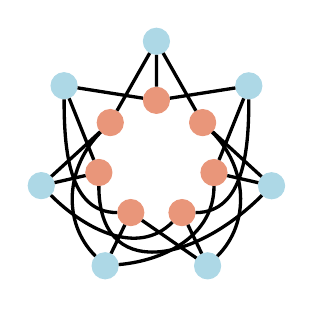
\begin{tikzpicture}[scale=0.75]

    \def\degree{51.42}
    \foreach \y/\colour in {1/lightred,2/lightblue}
    {
        \foreach \x in {0,...,6}
        {
            \node[vertex,\colour,fill=\colour] (p\y\x) at (\x*\degree+90:\y) {};
        }
    }\draw[edge] (p10) -- (p20) -- (p11) -- (p22) -- (p12) -- (p21) -- (p10) -- (p26) -- (p15) -- (p25) -- (p16) -- (p20);
    \path[edge] (p21) to[out=-90,in=180] (p13);
    \path[edge] (p13) -- (p24);
    \path[edge] (p24) to[out=45,in=-45] (p16);
    \draw[edge] (p26) to[out=-90,in=0] (p14);
    \draw[edge] (p14) to[out=-135,in=-45] (p22);
    \draw[edge] (p15) to[out=-90,in=5] (p23);
    \draw[edge] (p23) to[out=135,in=-135] (p11);
    \draw[edge] (p12) to[out=-90,in=-135,looseness=1.5] (p25);
    \draw[edge] (p13) -- (p23);
    \draw[edge] (p14) -- (p24);
\end{tikzpicture}
         \end{center}
        \subcaption{$\leviFano$.}
        \label{small-cc:leviFano/fig}
    \end{subfigure}
    \hfil
    \begin{subfigure}[]{.24\textwidth}
        \begin{center}
            

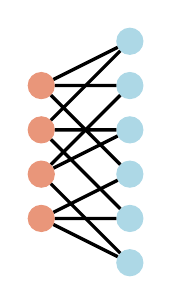
\begin{tikzpicture}[scale=0.75]

    \foreach \x in {0,...,3}
    {
        \node[vertex,lightred,fill=lightred] (r\x) at (0,3*\x/4) {};
    }
    \foreach \x in {0,...,5}
    {
        \node[vertex,lightblue,fill=lightblue] (b\x) at (1.5,3*\x/4-0.75) {};
    }
    \draw[edge] (r0) -- (b0) -- (r1) -- (b3) -- (r2) -- (b5) -- (r3) -- (b2) -- (r0);
    \draw[edge] (r0) -- (b1) -- (r2);
    \draw[edge] (r1) -- (b4) -- (r3);

\end{tikzpicture}
         \end{center}
        \subcaption{$\interspaceFourSix$.}
        \label{small-cc:graph-between-4cc-6cc/fig}
    \end{subfigure}
    \caption{Special graphs.}
    \label{small-cc:special-interspaces/fig}
\end{figure}

The incidence graph (or Levi graph) of the Fano plane~$\leviFano$ is a bipartite graph on two parts~$R$ and~$B$ each of size~$7$.
The set of arcs~$\arcs(\leviFano)$ is, up to isomorphism, determined by following property:
for each~$X \in \{R,B\}$ and~$v,v'\in X$ there is exactly one~$w \in (R \cup B) \setminus X$ for which~$vw,v'w \in \arcs(\leviFano)$.
The graph~$\leviFano$ is shown in Figure~\ref{small-cc:special-interspaces/fig}(\subref{small-cc:leviFano/fig}).
The graph~$\interspaceFourSix$ is the graph obtained form~$K_4$ by subdividing every edge.
It is a bipartite graph with vertex set~$R \disjointUnion B$ where~$\abs{R} = 4$ and~$\abs{B} = 6$.
For every~$\{r,r'\} \subsetneq R$ there is exactly one~$b \in B$ such that~$rb,r'b \in \arcs(\interspaceFourSix)$.
Figure~\ref{small-cc:special-interspaces/fig}(\subref{small-cc:graph-between-4cc-6cc/fig}) depicts~$\interspaceFourSix$.

 

\section{Critical Configurations}
\label{critical-graph/sec}

\begin{definition}
\label{def:critical-graph}
    We call a coherent configuration~$\coherentConfig$ \emph{critical} if~$\wldim{\coherentConfig}\geq 2$ and  there is no set of fibers~$\mathcal{R} \subsetneq \fibers{\coherentConfig}$ such that~$\wldim{\coherentConfig - \bigcup_{R \in \mathcal{R}} R} = \wldim{\coherentConfig}$.
\end{definition}


\begin{lemma}
\label{crictial:quotientGraph-connected/lem} \label{critical:disjoint-union/lem}
    Let~$\coherentConfig$ be a coherent configuration.
    If~$\coherentConfig$ is critical, then~$\quotientGraph{\coherentConfig}$ is connected.
\end{lemma}
\begin{proof}\textcolor{red}{TOPROVE 0}\end{proof}


\begin{lemma}
\label{critical:star/lem}
    Let~$\coherentConfig$ be a coherent configuration.
    If~$\coherentConfig$ is critical, then there are no distinct fibers~$R,B \in \fibers{\coherentConfig}$ with~$\minimalDegree{B}{R}=1$, that is, fibers with~$\disjointCliques{\abs{R}}{1,\frac{\abs{B}}{\abs{R}}} \in \interspace{R}{B}$.
\end{lemma}
\begin{proof}\textcolor{red}{TOPROVE 1}\end{proof}


\begin{lemma}
\label{critical:cycle/lem}
    Let~$\coherentConfig$ be a coherent configuration.
    If~$\coherentConfig$ is critical, then there are no fibers~$R,B\in \fibers{\coherentConfig}$ with~$|R|=|B|$ odd such that~$\minimalDegree{R}{B}=2$.
    In particular, if~$\coherentConfig$ is critical, then there is no interspace~$\disjointCycles{t}{2x} \in \interspace{R}{B}$ for positive integers~$t,x$ with~$x$ odd.
\end{lemma}
\begin{proof}\textcolor{red}{TOPROVE 2}\end{proof}


A fiber~$R$ of a coherent configuration is called~\emph{large} if~$8 \leq \abs{R}$, \emph{small} if~$4 \leq \abs{R} \leq 7$, and~\emph{tiny} if~$\abs{R} \leq 3$.
Thinking of red, blue and yellow, we will typically use the letters~$R$,~$B$ and~$Y$ for fibers in general. We will use~$L$ or~$S$ to indicate that the fiber in question is large or small, respectively.


\begin{lemma}
\label{critical:tiny-CC/lem}
    Let~$\coherentConfig$ be a coherent configuration.
    If~$\coherentConfig$ is critical, then there is no tiny fiber in~$\fibers{\coherentConfig}$.
\end{lemma}
\begin{proof}\textcolor{red}{TOPROVE 3}\end{proof}


Let~$\mathcal{R}$ be a union of fibers of~$\coherentConfig$, and let~$\mathcal{B}$ be the union of fibers that are not in~$\mathcal{R}$ but adjacent (in~$\quotientGraph{\coherentConfig}$) to some fiber in~$\mathcal{R}$.
We call~$\mathcal{R}$ \emph{restorable} if every automorphism of~$\coherentConfig[\mathcal{B}]$ that extends to an automorphism of
$\coherentConfig-\mathcal{R}$ also extends to an automorphism of~$\coherentConfig[\mathcal{R} \cup \mathcal{B}]$.


\begin{lemma}
\label{critical:restorable/lem}
    Let~$\coherentConfig$ be a coherent configuration.
    If~$\coherentConfig$ is critical, then there is no restorable union of fibers that is non-dominating.
\end{lemma}
\begin{proof}\textcolor{red}{TOPROVE 4}\end{proof}



Let~$R$ be a fiber of a coherent configuration. We say that a fiber~$Y$ distinct from~$R$ is \emph{taken care of (regarding restorability of~$R$)} if for every~$y\in Y$ and~$U\in \interspace{Y}{R}$ there is a fiber~$B$  different from~$R$ and~$Y$, a point~$b\in B$, and an interspace~$U_B\in \interspace{B}{R}$  such that~$bU_B\subseteq yU$.


\begin{lemma}
    \label{critical:restorable:take-care/lem}
    Let~$\coherentConfig$ be a coherent configuration with distinct fibers~$R$ and~$Y$.
    If~$Y$ is taken care of (regarding restorability of~$R$) and~$R$ is restorable in~$\coherentConfig-Y$, then~$R$ is restorable in~$\coherentConfig$.
\end{lemma}
\begin{proof}\textcolor{red}{TOPROVE 5}\end{proof}


We call a vertex set~$R \subseteq \vertices(\coherentConfig)$ a~\emph{module} if for all~$b \in \vertices(\coherentConfig) \setminus R$ and all~$\arcs \in \relations(\coherentConfig)$ we have~$b\arcs \cap R \in \{\emptyset, R\}$.


\begin{lemma}
\label{critical:small-cc:module/lem}
    Let~$\coherentConfig$ be a coherent configuration that is not homogeneous.
    If~$\coherentConfig$ is critical, then there is no small fiber that can be properly partitioned into at most 3 modules.
\end{lemma}
\begin{proof}\textcolor{red}{TOPROVE 6}\end{proof}


\begin{theorem}
\label{interspace-divisor/thm}
    Let~$\coherentConfig$ be a coherent configuration.
    Suppose~$(R,B,Y)$ is an induced path in~$\quotientGraph{\coherentConfig}$, $r \in R$, $y \in Y$, $U \in \interspace{R}{B}$, and~$U' \in \interspace{Y}{B}$.
    Then~$\intDegree{U} \cdot \intDegree{U'} = \abs{B} \cdot \abs{rU \cap yU'}$.

    In particular~$\lcm\{\abs{B}, \intDegree{U}\}>1$ and~$\lcm\{\abs{B}, \intDegree{U'}\}>1$. In particular~$\abs{B}$ is not prime.
\end{theorem}
\begin{proof}\textcolor{red}{TOPROVE 7}\end{proof}
     

\section{Small fibers and their interspaces}
\label{small-cc/sec}


Given an interspace~$\interspace{R}{B}$ between the fibers~$R$ and~$B$, define~$\type{\interspace{R}{B}}$ to be the collection of basis relations~$\arcs$ in a~$\interspace{R}{B}$ up to isomorphism while omitting transpose basis relation~$\arcs^\star$,~$1_R$, and~$1_B$.




\begin{table}
    \centering\def\arraystretch{1.5}\begin{tabular}{|c|l|}
        \hline
        $\abs{R}$ & $\type{\inducedCC{R}}$ \\ \hline
        1 & $(K_1)$\\ \hline
        2 & $(K_2)$\\ \hline
        3 & $(K_3)$\\ \hline
        4 & $(K_4)$,~$(C_4,2K_2)$,~$(2K_2,2K_2,2K_2)$,~$(\overrightarrow{C_4},2K_2)$\\ \hline
        5 & $(K_5)$,~$(C_5,C_5)$,~$(\overrightarrow{C_5},\overrightarrow{C_5})$, \\ \hline
        6 & $(K_6)$,~$(2 K_3,K_{3,3})$,~$(2\overrightarrow{C_3},K_{3,3})$,~$(3 K_2,K_{2,2,2})$,~$(3K_2,\overrightarrow{C_3}[K_2])$,\\
            & $(C_6,3K_2,2K_3)$,~$(\overrightarrow{C_6},2\overrightarrow{C_3},3K_2)$,~$(3K_2,3K_2,\overrightarrow{2C_3},3K_2)$\\ \hline
        7 & $(K_7)$,~$(C_7,C_7,C_7)$,~$(PTr(7))$,~$(\overrightarrow{C_7},\overrightarrow{C_7},\overrightarrow{C_7})$ \\ \hline
    \end{tabular}
    \caption{Classification of all homogeneous coherent configuration of order~$n \leq 7$.}
    \label{small-cc:classificaiton-small-cc/tab}
\end{table}
 

\begin{lemma}
\label{small-cc:induced-cc/lem} \label{small-cc:implied-cc/lem}
    Every small fiber~$R$ in a coherent configuration induces, up to isomorphism, one of 22 coherent configurations. These 22 options are given in Table~\ref{small-cc:classificaiton-small-cc/tab}.
\end{lemma}
\begin{proof}\textcolor{red}{TOPROVE 8}\end{proof}


Note that for small fibers, the constituents of the induced homogeneous coherent configuration contained within a fiber determine the isomorphism type of said homogeneous coherent configuration.
(This is not necessarily the case for larger fibers.)


\begin{figure}[tbp]
    \centering
    \begin{subfigure}[]{.23\textwidth}
        \begin{center}
            

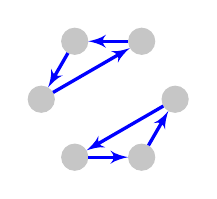
\begin{tikzpicture}[scale=0.85]

    \def\degree{60}

    \foreach \x in {0,...,5}
    {
        \node[vertex,lightgray,fill=lightgray] (p\x) at (\x*\degree+60:1) {};
    }
    \draw[arrow,blue]
        (p0) edge (p1)
        (p1) edge (p2)
        (p2) edge (p0);
    \draw[arrow,blue]
        (p3) edge (p4)
        (p4) edge (p5)
        (p5) edge (p3);
\end{tikzpicture}
         \end{center}
        \subcaption{$(2\overrightarrow{C_3},K_{3,3})$.}
        \label{small-cc:6cc:directed-2K3/fig}
    \end{subfigure}
    \hfil
    \begin{subfigure}[]{.23\textwidth}
        \begin{center}
            

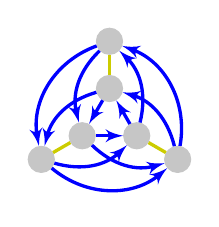
\begin{tikzpicture}[scale=0.4]
    \node[vertex,lightgray,fill=lightgray] (p0) at (90:1) {};
    \node[vertex,lightgray,fill=lightgray] (p1) at (90:2.5) {};
    \node[vertex,lightgray,fill=lightgray] (p2) at (210:1) {};
    \node[vertex,lightgray,fill=lightgray] (p3) at (210:2.5) {};
    \node[vertex,lightgray,fill=lightgray] (p4) at (330:1) {};
    \node[vertex,lightgray,fill=lightgray] (p5) at (330:2.5) {};
    \draw[arrow,blue]
        (p0) edge (p2)
        (p2) edge (p4)
        (p4) edge (p0);
    \draw[arrow,blue, bend right=40]
        (p1) edge (p3)
        (p3) edge (p5)
        (p5) edge (p1);
    \draw[arrow,blue, bend right]
        (p0) edge (p3)
        (p3) edge (p4)
        (p4) edge (p1)
        (p1) edge (p2)
        (p2) edge (p5)
        (p5) edge (p0);

    \draw[edge,darkyellow] (p0) -- (p1);
    \draw[edge,darkyellow] (p2) -- (p3);
    \draw[edge,darkyellow] (p4) -- (p5);

\end{tikzpicture}
         \end{center}
        \subcaption{$(\overrightarrow{C_3}[K_2],3K_2)$.}
        \label{small-cc:6cc:wreath/fig}
    \end{subfigure}
    \hfil
    \begin{subfigure}[]{.27\textwidth}
        \begin{center}
            

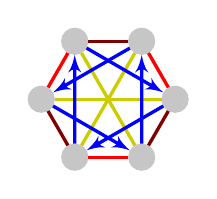
\begin{tikzpicture}[scale=0.85]

    \def\degree{60}

    \foreach \x in {0,...,5}
    {
        \node[vertex,lightgray,fill=lightgray] (p\x) at (\x*\degree+60:1) {};
    }
    \draw[edge,darkred] (p0) -- (p1);
    \draw[edge,darkred] (p2) -- (p3);
    \draw[edge,darkred] (p4) -- (p5);

    \draw[edge,red] (p1) -- (p2);
    \draw[edge,red] (p3) -- (p4);
    \draw[edge,red] (p5) -- (p0);

    \draw[edge,darkyellow]
        (p0) edge (p3)
        (p1) edge (p4)
        (p5) edge (p2);

    \draw[arrow,blue]
        (p0) edge (p2)
        (p2) edge (p4)
        (p4) edge (p0);
    \draw[arrow,blue]
        (p1) edge (p5)
        (p5) edge (p3)
        (p3) edge (p1);
\end{tikzpicture}
         \end{center}
        \subcaption{$(3K_2,3K_2,2\overrightarrow{C_3},3K_2)$.}
        \label{small-cc:6cc:alternating-C6/fig}
    \end{subfigure}
    \hfil
    \begin{subfigure}[]{.23\textwidth}
        \begin{center}
            

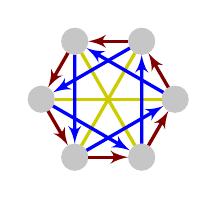
\begin{tikzpicture}[scale=0.85]

    \def\degree{60}

    \foreach \x in {0,...,5}
    {
        \node[vertex,lightgray,fill=lightgray] (p\x) at (\x*\degree+60:1) {};
    }
    \draw[arrow,darkred]
        (p0) edge (p1)
        (p1) edge (p2)
        (p2) edge (p3)
        (p3) edge (p4)
        (p4) edge (p5)
        (p5) edge (p0);

    \draw[edge,darkyellow] (p0) -- (p3);
    \draw[edge,darkyellow] (p1) -- (p4);
    \draw[edge,darkyellow] (p5) -- (p2);

    \draw[arrow,blue]
        (p0) edge (p2)
        (p2) edge (p4)
        (p4) edge (p0);
    \draw[arrow,blue]
        (p1) edge (p3)
        (p3) edge (p5)
        (p5) edge (p1);
\end{tikzpicture}
         \end{center}
        \subcaption{$(\overrightarrow{C_6},2\overrightarrow{C_3},3K_2)$.}
        \label{small-cc:6cc:directed-C6/fig}
    \end{subfigure}
    \caption{Coherent configurations of order~$6$ with directed edges.}
    \label{small-cc:6cc:coherent-config/fig}
\end{figure}


\begin{lemma}
    \label{small-cc:interspace/lem}
    Let~$\coherentConfig$ be a coherent configuration, and let~$(R,B)$ be an edge in~$\quotientGraph{\coherentConfig}$ such that~$2 \leq \abs{R} \leq \abs{B} \leq 7$.
    \begin{enumerate}[label=(\arabic*)]
        \item If~$\abs{R} = 2$,
        then~$\abs{B} \in \{2,4,6\}$ and~$\disjointCliques{2}{1,\frac{\abs{B}}{2}} \in \interspace{R}{B}$.
        \item If~$\abs{R} = 3$,
        then~$\abs{B} \in \{3,6\}$ and~$\disjointCliques{3}{1,\frac{\abs{B}}{2}} \in \interspace{R}{B}$.
        \item If~$\abs{R} = 4$, then~$\abs{B} \in \{4,6\}$.
        Furthermore, if~$\abs{R} = 4$ and~$\abs{B} = 4$, then at least one of the constituents~$\cycle{8}$, $\matching{4}$, and~$\disjointCliques{2}{2,2}$ is contained in~$\interspace{R}{B}$, and if~$\abs{R} = 4$ and~$\abs{B} = 6$, then at least one of constituents~$\interspaceFourSix$ and~$\disjointCliques{2}{2,3}$ is contained in~$\interspace{R}{B}$.
        \item If~$\abs{R} = 5$,
        then~$\abs{B} = 5$ and~$\matching{5} \in \interspace{R}{B}$.
        \item If~$\abs{R} = 6$,
        then~$\abs{B} = 6$ and at least one of constituents~$\matching{6}$, $\cycle{12}$, $\disjointCliques{3}{2,2}$, or~$\disjointCliques{2}{3,3}$ is contained in~$\interspace{R}{B}$.
        \item If~$\abs{R} = 7$,
        then~$\abs{B} = 7$ and at least one of constituents~$\matching{7}$ and~$\leviFano$ is contained in~$\interspace{R}{B}$.
    \end{enumerate}
\end{lemma}
\begin{proof}\textcolor{red}{TOPROVE 9}\end{proof}




\begin{table}
    \centering\def\arraystretch{1.2}\begin{tabular}{|c|c|l|}
        \hline
        $\abs{R}$ & $\abs{B}$ & $\type{\interspace{R}{B}}$ \\ \hline
        4 & 4 & $(\cycle{8}, \cycle{8})$, $(\disjointCliques{2}{2,2}, \disjointCliques{2}{2,2})$\\ \hline
        4 & 6 & $(\interspaceFourSix, \interspaceFourSix)$, $(\disjointCliques{2}{2,3},\disjointCliques{2}{2,3})$\\ \hline
        6 & 6 & $(\cycle{12}, \cycle{12}, \disjointCliques{3}{2,2})$, $(\disjointCliques{2}{3,3},\disjointCliques{2}{3,3})$, $(\disjointCliques{3}{2,2}, \disjointCliques{3}{2,2}, \disjointCliques{3}{2,2})$, $(\disjointCliques{3}{2,2},R \times B - \disjointCliques{3}{2,2})$ \\ \hline
        7 & 7 & $(\leviFano, R \times B -\leviFano)$ \\ \hline
    \end{tabular}
    \caption{Classification of all~$\interspace{R}{B}$ with~$2 \leq \abs{R} \leq \abs{B} \leq 7$ in critical coherent configurations.}
    \label{small-cc:classificaiton-small-interspaces/tab}
\end{table}
 

To classify all possible isomorphism types of interspaces between small fibers, we can examine the coarsest coherent configurations containing one of the graphs guaranteed to exists by Lemma~\ref{small-cc:interspace/lem} as constituent. Table~\ref{small-cc:classificaiton-small-interspaces/tab} lists all isomorphism types between two small fibers in a critical coherent configuration. Note that the isomorphism type is determined by the isomorphism types of its constituents. (This is not necessarily the case for interspaces between larger fibers). For fibers of size~$4$ and~$6$ the classification can alternatively derived from the upcoming Theorem~\ref{global-argument:large-small-interspace:classification}.


\begin{lemma}
\label{small-cc:interspace-implies-cc/lem}
    Let~$\coherentConfig$ be a coherent configuration, and let~$(R,B)$ be an edge in~$\quotientGraph{\coherentConfig}$ with~$\abs{R} \leq \abs{B}$, and suppose~$x \in \{4,6\}$ and~$y \in \{2,3\}$.
    \begin{enumerate}[label = (\arabic*)]
        \item
        If~$\cycle{2x} \in \interspace{R}{B}$, then~$\cycle{x} \in \inducedCC{R}$.
        \item
        If~$y\clique{2,2} \in \interspace{R}{B}$, then~$\disjointCliques{y}{2} \in \inducedCC{R}$.
        \item
        If~$\disjointCliques{2}{2,3} \in \interspace{R}{B}$, then~$\matchingCC{2} \in \inducedCC{R}$ and either~$\disjointCliques{2}{3} \in \inducedCC{B}$ or~$2\overrightarrow{C_3} \in \inducedCC{B}$.
        \item
        If~$\disjointCliques{2}{3,3} \in \interspace{R}{B}$, then either~$\disjointCliques{2}{3} \in \inducedCC{R}$ or~$2\overrightarrow{\cycle{3}} \in \inducedCC{B}$.
        \item
        If~$\leviFano \in \interspace{R}{B}$, then either~$\clique{7} \in \inducedCC{R}$ or~$PTr(7) \in \inducedCC{R}$.
        \item
        If~$\interspaceFourSix \in \interspace{R}{B}$, then~$\clique{4} \in \inducedCC{R}$ and either~$\matchingCC{3}, K_{2,2,2} \in \inducedCC{B}$ or~$\matchingCC{3},\overrightarrow{\cycle{3}}[\clique{2}] \in \inducedCC{B}$.
    \end{enumerate}
\end{lemma}
\begin{proof}\textcolor{red}{TOPROVE 10}\end{proof}




     

\section{Interspaces between large and small fibers}
\label{interspace-large-small/sec}

To study interspaces between large and small fibers we will introduce a specialized notation that concisely captures the attachment structure that vertices in the large fiber have in the small fiber.
The challenge is to capture the entire information for all constituents simultaneously.

For a relation~$\arcs$, we define~$\ul(\arcs)$ to be~$\arcs \cup \arcs^\star$.
We extend this notation to graphs and coherent configurations to obtain their \emph{underlying undirected structure}.
For a coherent configuration~$\coherentConfig$, we set~$\ul(\coherentConfig)$ to be~$(\vertices(\coherentConfig), \{\ul(\arcs) \mid \arcs \in \relations(\coherentConfig)\})$.
Observe that~$\ul(\coherentConfig)$ is not necessarily coherent.
For a graph~$G$, we set~$\ul(G)$ to be~$(\vertices(G), \ul(\arcs(G)))$ and call it the \emph{underlying undirected graph} of~$G$.

Let~$L,S$ be distinct fibers of a coherent configuration~$\coherentConfig$.
We say the interspace~$\interspace{L}{S}$ contains the \emph{interspace pattern} $(G^1, d^1_1, d^1_2, \dots, d^1_{t_1}; \dots; G^k, d^k_1, d^k_2, \dots, d^k_{t_k})$ if~$\sum_{j = 1}^{k} t_j = \abs{\interspace{L}{S}} - 1$, there are distinct~$\arcs^1, \dots, \arcs^k \in \inducedCC{S}$ such that for each~$i \in \{1,\dots,k\}$ we have~$\ul(S,\arcs^i) \cong G^i$, and there are distinct~$U^i_1, \dots, U^i_{t_i} \in \interspace{L}{S}$ such that for all~$\ell \in L$ and~$j \in \{1, \dots, t_i\}$ the set~$\ell U^i_j$ induces a~$d^i_j$-clique in~$\ul(S,A^i)$. We should emphasize that the sum of the~$t_i$ is~$\abs{\interspace{L}{S}} - 1$ and thus we omit exactly one of the interspaces in the pattern. In fact, in general the missing interspace will not satisfy a clique condition. Also, it is a priori not clear that an interspace always has a pattern of this form we just defined.

Considering~$d^i_j = 3$, if for all~$S' \subseteq S$ that induce a~$3$-clique in~$\ul(S,A^1)$ the common neighborhood~$\bigcap_{s \in S'} s {U^i_j}^\star$ is not empty, then we mark the entry in the interspace pattern by~$^\dag$. This means there is a vertex in~$\ell\in L$ such that~$\ell U^i_j= S'$.
On the other hand, if  for all~$S' \subseteq S$ inducing a~$3$-clique in~$\ul(S,A^1)$ we have that~$S\setminus S'$ is a also~$3$-clique and exactly one of~$\bigcap_{s \in S'} s {U^i_j}^\star$ or~$\bigcap_{s \in S \setminus S'} s {U^i_j}^\star$ is not empty, then we mark the entry by~$^\ddag$.
For example, the interspace pattern~$(\clique{2,2,2},3)$ has two subpatterns, namely~\ipsixMatchingComplement\xspace and~\ipsixMatchingComplementD. In principle there could be other subcases, but it will follow from our classification that only these two subcases arise.


\begin{theorem}
\label{global-argument:large-small-interspace:classification}
    Let~$\coherentConfig$ be a critical coherent configuration and~$(L,S)$ be an edge in~$\quotientGraph{\coherentConfig}$.
    If~$\abs{S} \in \{4,6\}$, then~$\interspace{L}{S}$ contains one of the following interspace patterns:
    \begin{multicols}{4}
        \begin{enumerate}
            \item \ipfourClique
            \item \ipfourMatching
            \item \ipfourCycle
            \item \ipsixCliqueTwo
            \item \ipsixCliqueTwoTwice
            \item \ipsixMatching
            \item \ipsixMatchingTwice
            \item \ipsixMatchingAndCycle
            \item \ipsixMatchingMatching
            \item \ipsixMatchingAndComplement
            \item \ipsixTriangleComplement
            \item \ipsixTriangleComplementTwice
            \item \ipsixCliqueThree
            \item \ipsixCliqueThreeD
            \item \ipsixTriangle
            \item \ipsixMatchingComplement
            \item \ipsixMatchingComplementD.
        \end{enumerate}
    \end{multicols}
\end{theorem}
\begin{proof}\textcolor{red}{TOPROVE 11}\end{proof}


We can observe that the interspace patterns in the theorem are mutually exclusive, and we conclude the following.


\begin{corollary}
\label{large-small-interspace:classification:uniqueness/cor}
    Let~$\coherentConfig$ be a critical coherent configuration, and let~$(L,S)$ be an edge in~$\quotientGraph{\coherentConfig}$.
    If~$\abs{S} \in \{4,6\}$, then~$\interspace{L}{S}$ contains \underline{exactly} one of interspace patterns listed in Theorem~\ref{global-argument:large-small-interspace:classification}.
\end{corollary}
\begin{proof}\textcolor{red}{TOPROVE 12}\end{proof}

We should stress that this classification of the interspaces between fibers~$L$ and~$S$ on interspace pattern is only possible because we consider small fibers with~$S$ of size~$4$ or~$6$.


For an interspace pattern~$\mathfrak{P}$ of~$\interspace{L}{S}$ we write~$A^i(\interspace{L}{S})$ and~$U^i_j(\interspace{L}{S})$ to denote~$A^i$ and~$U^i_j$ as given in the definition of interspace pattern. While the interspace pattern~$\mathfrak{P}$ is unique for interspace~$\interspace{L}{S}$, the choice for~$A^i$ is only determined up to isomorphism. For a given coherent configuration we will always choose an arbitrary but fixed~$A^i$ and matching~$U^i_j$.


\begin{lemma}
\label{global-argument:k4-exclusion/lem}
    Let~$\coherentConfig$ be a critical coherent configuration and~$(R,Y,B)$ a path in~$\quotientGraph{\coherentConfig}$.
    If either~$\clique{4} \in \inducedCC{Y}$ or~$\clique{6} \in \inducedCC{Y}$, then~$\interspace{R}{B}$ is not homogeneous.
\end{lemma}
\begin{proof}\textcolor{red}{TOPROVE 13}\end{proof}


Let~$(G^1, d^1_1, d^1_2, \dots, d^1_{t_1}; \dots; G^k, d^k_1, d^k_2, \dots, d^k_{t_k})$ be the interspace pattern of~$\interspace{L}{S}$, and let~$i \in \{1,\ldots,k\}$ and~$j \in \{1,\ldots,t_i\}$.
For~$U = U^i_j(\interspace{L}{S})$, two vertices~$\ell, \ell' \in L$ are called \emph{equivalent} with respect to~$S$ and~$U$ if~$\ell U =\ell'U$.
We denote the set of all equivalence classes with respect to~$S$ and~$U^i_j(\interspace{L}{S})$ by~$\partitionRel{i}{j}{L,S}$.
Further, we define~
\[
    \equivalenceClasses{L,S} \coloneqq \bigwedge_{\substack{i \in \{1,\ldots,k\} \\ j \in \{1,\ldots,t_i\}}}  \partitionRel{i}{j}{L,S},
\]
that is,~$\equivalenceClasses{L,S}$ is  the meet of all partitions~$\partitionRel{i}{j}{L,S}$.
In other words,~$\equivalenceClasses{L,S}$ is the coarsest partition which still finer than all~$\partitionRel{i}{j}{L,S}$. Also not that~$\equivalenceClasses{L,S} = \partition{L,S}$ if~$|\interspace{L}{S}|=2$.
For a union of small fibers~$\mathcal{S}$, we define~$\equivalenceClasses{L,\mathcal{S}} \coloneqq \bigwedge_{S \in \mathcal{S}} \equivalenceClasses{L,S}$.


\begin{lemma}
\label{interspace-pattern:partition-size/lem}
    Let~$\coherentConfig$ be a critical coherent configuration, $(L,S)$ an edge in~$\quotientGraph{\coherentConfig}$ with~$|S|\in \{4,6\}$ and suppose that~$\interspace{L}{S}$ has interspace pattern~$(G^1, d^1_1, \dots, d^1_{t_1}; \dots; G^k, d^k_1, \dots, d^k_{t_k})$.
    Let~$x$ be the number of $3$-cliques in~$G^1$.

    Then~$\abs{\partition{L,S}} = \abs{A^1(\interspace{L}{S})}$ if~$d^1_1 = 2$, $\abs{\equivalenceClasses{L,S}} = x$ if~$d^1_1 = 3^\dag$, and~$\abs{\equivalenceClasses{L,S}} = \frac{x}{2}$ if~$d^1_1 = 3^\ddag$.
\end{lemma}
\begin{proof}\textcolor{red}{TOPROVE 14}\end{proof}


Table~\ref{interspace-pattern:partition-size/tab} gives an explicit overview of how the partition size~$\abs{\partition{L,S}}$ depends on the interspace patterns of Theorem~\ref{global-argument:large-small-interspace:classification}.




\begin{table}[tbp]
    \centering\def\arraystretch{1.2}\begin{tabular}{|c|l|}
        \hline
        $\abs{\partition{L,S}}$ & interspace pattern contained in~$\interspace{L}{S}$                   \\ \hline
        $2$                     & $\ipfourMatching$, $\ipsixTriangle$                                   \\ \hline
        $3$                     & $\ipsixMatching$, $\ipsixMatchingTwice$, $\ipsixMatchingMatching$     \\ \hline
        $4$                     & $\ipfourCycle$, $\ipsixMatchingComplementD$                           \\ \hline
        $6$                     & $\ipsixMatchingAndCycle$, $\ipfourClique$                             \\ \hline
        $8$                     & $\ipsixMatchingComplement$                                            \\ \hline
        $9$                     & $\ipsixTriangleComplement$, $\ipsixTriangleComplementTwice$           \\ \hline
        $10$                    & $\ipsixCliqueThreeD$                                                  \\ \hline
        $12$                    & $\ipsixMatchingAndComplement$                                         \\ \hline
        $15$                    & $\ipsixCliqueTwo$, $\ipsixCliqueTwoTwice$                             \\ \hline
        $20$                    & $\ipsixCliqueThree$                                                   \\ \hline
    \end{tabular}
    \caption{Overview of~$\abs{\partition{L,S}}$ depending on the interspace pattern in~$\interspace{L}{S}$.}
    \label{interspace-pattern:partition-size/tab}
\end{table}

 

\begin{lemma}
\label{global-argument:partition:fully-intersecting/lem}
    Let~$\coherentConfig$ be a coherent configuration, and~$(R_1, L, R_2)$ a path in~$\quotientGraph{\coherentConfig}$.
    If~$\abs{\partition{L,R_1}}$ and~$\abs{\partition{L,R_2}}$ are coprime, then partitions~$\partition{L,R_1}$ and~$\partition{L, R_2}$ are \emph{fully intersecting}, that is, $P_1 \cap P_2 \neq \emptyset$ for all~$P_1 \in \partition{L,R_1}, P_2 \in \partition{L,R_2}$.
\end{lemma}
\begin{proof}\textcolor{red}{TOPROVE 15}\end{proof}



Let~$\mathcal{S}$ be a union of small fibers each adjacent to a large fiber~$L$ in the quotient graph of a coherent configuration~$\coherentConfig$.
For~$U,U' \in \interspace{L}{\mathcal{S}}$, we define a function~$\eta_{U,U'} \colon \equivalenceClasses{L,\mathcal{S}}^2 \longrightarrow \Nat$ with~$(P,P') \mapsto | p U \cap p' U'|$ where~$p \in P,p' \in P'$ are arbitrary.
We define~$\mathcal{Q}$ to be the set of equivalence classes on~$\equivalenceClasses{L,S}^2$ such that for all~$Q \in \mathcal{Q}$ we have
\[
    (P_1,P_2),(P'_1,P'_2) \in Q \text{ if and only if } \eta_{U,U'}(P_1,P_2) = \eta_{U,U'}(P'_1,P'_2) \text{ for all } U,U' \in \interspace{L}{\mathcal{S}}.
\]
We call the coherent configuration~$(\equivalenceClasses{L,\mathcal{S}}, \mathcal{Q})$ the~\emph{partition structure}, denoted by~$\partitionStructure{L,\mathcal{S}}$.
Intuitively speaking, the vertices of the partition structure correspond to the parts of $\equivalenceClasses{L,\mathcal{S}}$. For the arcs between a pair of parts, the relations represent what the arcs in~$L$ ``know'' about the intersection of common neighborhoods of their end vertices in~$\mathcal{S}$ (with respect to basis relations in~$\interspace{L}{\mathcal{S}}$).
Observe that~$\partitionStructure{L,\mathcal{S}}$ is indeed a coherent configuration itself.




\begin{table}[tb]
    \centering\def\arraystretch{1.5}\begin{tabular}{|l|l|l|}
        \hline
        \makecell{Interspace pattern \\ of~$\interspace{L}{S}$} & $\type{\inducedCC{S}}$                                                                                                                                                                    & $\type{\partitionStructure{L,S}}$                                     \\ \hline
        $\ipfourClique$                                         & $(K_4)$                                                                                                                                                                                   & $(3K_2,K_{2,2,2})$                                                    \\ \hline
        $\ipfourMatching$                                       & $(2K_2,2K_2,2K_2)$, $(C_4,2K_2)$, $(\overrightarrow{C_4},2K_2)$                                                                                                                           & $(K_2)$                                                              \\ \hline
        $\ipfourCycle$                                          & $(2K_2,C_4)$                                                                                                                                                                              & $(2K_2,C_4)$                                                          \\ \hline
        $\ipsixMatching$                                        & $(3K_2,K_{2,2})$, $(C_6,2C_3,3K_2)$,                                                                                                                                                      & $(K_3)$                                                              \\ \hline
        \multirow{2}{*}{$\ipsixMatchingTwice$}                  & $(3K_2,K_{2,2,2})$, $(C_6,2C_3,3K_2)$,                                                                                                                                                      & $(3K_2,3K_2,2\overrightarrow{C_3},3K_2)$                                                    \\ \cline{2-3}
                                                                & $(3K_2,\overrightarrow{C_3}[K_2])$, $(\overrightarrow{C_6},2\overrightarrow{C_3},3K_2)$                                                                                                   & $(\overrightarrow{C_3})$                                              \\ \hline
        $\ipsixMatchingAndCycle$                                & $(C_6,2C_3,3K_2)$                                                                                                                                                                         & $(C_6,2C_3,3K_2)$                                                     \\ \hline
$\ipsixTriangleComplement    $                          & $(2K_3,K_{3,3})$                                                                                                                                                                          & $(\rookGraph{3},\rookGraph{3})$                                       \\ \hline
\multirow{2}{*}{$\ipsixTriangle$}                       & $(2C_3,K_{3,3})$, $(2\overrightarrow{C_3},K_{3,3})$, $(C_6,2C_3,3K_2)$,                                                                                                                   & \multirow{2}{*}{$(K_2)$}                                             \\
                                                                & $(\overrightarrow{C_6},2\overrightarrow{C_3},3K_2)$, $(3K_2,3K_2,\overrightarrow{2C_3},3K_2)$                                                                                             &                                                                       \\ \hline
        $\ipsixMatchingMatching$                                & $(3K_2,3K_2,\overrightarrow{2C_3},3K_2)$                                                                                                                                                  & $(C_3)$                                                               \\ \hline
        $\ipsixMatchingComplement    $                          & $(3K_2,K_{2,2,2})$, $(3K_2,\overrightarrow{C_3}[K_2])$                                                                                                                                    & $(2K_4,4K_2,K_{4,4}-4K_2)$                                            \\ \hline
        $\ipsixMatchingComplementD    $                         & $(3K_2,K_{2,2,2})$, $(3K_2,\overrightarrow{C_3}[K_2])$                                                                                                                                    & $(K_4)$                                                               \\ \hline
    \end{tabular}
    \caption{Partition structure~$\partitionStructure{L,S}$ determined~$\inducedCC{S}$ and~$\interspace{L}{S}$ in a critical coherent configuration~$\coherentConfig$.}
    \label{interspace-pattern:partition-structure/tab}
\end{table}
 

\begin{lemma}
\label{interspace-pattern:partition-structure/lem}
    Let~$\coherentConfig$ be a critical coherent configuration and~$L,S \in \fibers{\coherentConfig}$.
    For~$|\partition{L,S}| \leq 8$, the coherent configuration~$\inducedCC{S}$ together with the interspace pattern of~$\interspace{L}{S}$ uniquely determines the partition structure~$\partitionStructure{L,S}$.
\end{lemma}
\begin{proof}\textcolor{red}{TOPROVE 16}\end{proof}


We should comment that the interspace pattern and the isomorphism type of the small fiber~$S$ does not uniquely determine the partition structure~$\partitionStructure{L,S}$ if~$|\partition{L,S}| \geq 9$.
Further, we remark that in a critical coherent configuration the interspace pattern might restrict the possible constituents in the small fiber, as we have shown in the proof of Theorem~\ref{large-small-interspace:classification:uniqueness/cor}:
For example, if an interspace~$\interspace{L}{S}$ has interspace pattern~$\ipfourCycle$ or~$\ipsixMatchingAndCycle$, then by coherence~$\overrightarrow{C_4} \notin \inducedCC{S}$ (respectively~$\overrightarrow{C_6} \notin \inducedCC{S}$) since~$U^1_1(\interspace{L}{S})$ would not be a basis relation.
For similar reasons~$2\overrightarrow{C_3} \notin \inducedCC{S}$ if~$\interspace{L}{S}$ has interspace pattern~$\ipsixTriangleComplement$.
For each interspace pattern and isomorphism type of configuration~$\inducedCC{S}$, the possible partition structures in a critical coherent configuration~$\coherentConfig$ are listed in Table~\ref{interspace-pattern:partition-structure/tab}.
     

\section{Restorable fibers}
\label{critical:restorable/sec}


\begin{lemma}
    \label{critical:adjacent-interspace-cycle/lem}
    Let~$\coherentConfig$ be a critical coherent configuration, and~$(R,S,Y)$ be a path in~$\quotientGraph{\coherentConfig}$ with~$S$ being small.
    \begin{enumerate}
        \item If both~$\interspace{R}{S}$ and~$\interspace{Y}{S}$ have interspace pattern~$\ipfourCycle$, then there is a union~$\arcs$ of basis relations in~$\interspace{R}{Y}$ such that~$(R \disjointUnion Y,\arcs) \cong \disjointCliques{4}{\frac{\abs{R}}{4},\frac{\abs{Y}}{4}}$.
        \item If both~$\interspace{R}{S}$ and~$\interspace{Y}{S}$ have interspace pattern~$\ipsixMatchingAndCycle$, then there is a union~$\arcs$ of basis relations in~$\interspace{R}{Y}$ such that $(R \disjointUnion Y,\arcs) \cong \disjointCliques{6}{\frac{\abs{R}}{6},\frac{\abs{Y}}{6}}$.
    \end{enumerate}
    In particular, fibers~$R$ and~$Y$ are large.
\end{lemma}
\begin{proof}\textcolor{red}{TOPROVE 17}\end{proof}


\begin{lemma}
    \label{critical:4cc:restorable:2,C4/lem}
    Let~$\coherentConfig$ be a critical coherent configuration and~$S \in \fibers{\coherentConfig}$ be a size-$4$ fiber.
    If~$\{S\}$ is not dominating and~$|\ul(\inducedCC{S})| = 3$, then there are fibers~$R,R'$ adjacent to~$S$ in~$\quotientGraph{\coherentConfig}$ such that~$\interspace{R}{S}$ has interspace pattern~$\ipfourCycle$ and~$\interspace{R'}{S}$ has interspace pattern~$\ipfourMatching$.
\end{lemma}
\begin{proof}\textcolor{red}{TOPROVE 18}\end{proof}


The \emph{color-disjoint union~$\coherentConfig$} of two coherent configurations~$\coherentConfig_1$ and~$\coherentConfig_2$ is the coherent configuration~$(\vertices(\coherentConfig_1) \disjointUnion \vertices(\coherentConfig_2), \arcs(\coherentConfig_1) \cup \arcs(\coherentConfig_2) \cup \{\vertices(\coherentConfig_1) \times \vertices(\coherentConfig_2)\})$.
Observe that~$\vertices(\coherentConfig_i) \in \fibers{\coherentConfig}^\cup$ for all~$i \in \{1,2\}$.
Thus there is no automorphism of~$\coherentConfig$ which maps~$\vertices(\coherentConfig_1)$ to~$\vertices(\coherentConfig_2)$ and vice versa.


\begin{lemma}
\label{critical:4cc:restorable:cycle/lem}
    Let~$\coherentConfig$ be critical coherent configuration, and let~$R_0,R_1 \in \fibers{\coherentConfig}$ be distinct.
    If~$\{R_0 , R_1\}$ is not dominating, then~$\cycle{8} \notin \interspace{R_0}{R_1}$.
\end{lemma}
\begin{proof}\textcolor{red}{TOPROVE 19}\end{proof}


\begin{lemma}
\label{critical:4-cc:restorable:DUC/lem}
    Let~$\coherentConfig$ be a critical coherent configuration and~$S \in \fibers{\coherentConfig}$ a fiber that is not dominating.
    For every~$\arcs \in \inducedCC{S}$ with~$(S,\arcs) \cong \disjointCliques{2}{2}$ there are~$R \in \fibers{\coherentConfig}$ and~$U \in \interspace{R}{S}$ such that for all~$r \in R$ the set~$r U$ induces a~$2$-clique in~$(S,\arcs)$.

    In particular, if~$\coherentConfig$ is critical and~$\ul(\inducedCC{S})| = 4$, then~$\colorDeg{S} \geq 3$.
\end{lemma}
\begin{proof}\textcolor{red}{TOPROVE 20}\end{proof}


\begin{lemma}
\label{6-cc:implied-interspace:DUC-DUC/lem}
    Let~$\coherentConfig$ be a coherent configuration, and let~$(R,B,Y)$ be path in~$\quotientGraph{\coherentConfig}$ with~$\abs{B} = 6$.
    \begin{enumerate}
        \item
        If~$\disjointCliques{3}{\frac{\abs{R}}{3},2} \in \interspace{R}{B}$ and~$\disjointCliques{3}{\frac{\abs{Y}}{3},2} \in \interspace{Y}{B}$,
        then there is a union~$U$ of relations in~$\coherentConfig$ such that~$(R \disjointUnion Y, U) \cong \disjointCliques{3}{\frac{\abs{R}}{3},\frac{\abs{Y}}{3}}$.

        \item
        If both~$\interspace{R}{B}$ and~$\interspace{Y}{B}$ have interspace pattern~$\ipsixTriangle$,
        then there is a union~$U$ of relations in~$\coherentConfig$ such that~$(R \disjointUnion Y, U) \cong \disjointCliques{2}{\frac{\abs{R}}{2},\frac{\abs{Y}}{2}}$.
    \end{enumerate}
\end{lemma}
\begin{proof}\textcolor{red}{TOPROVE 21}\end{proof}


For the convenience of the reader, Table~\ref{6-cc:implied-interspace:DUC-DUC/tab} gives an overview of the results of Lemmas~\ref{critical:adjacent-interspace-cycle/lem} and~\ref{6-cc:implied-interspace:DUC-DUC/lem} for size~$6$ fibers.




\begin{table}[tbp]
    \centering\def\arraystretch{1.2}\begin{tabular}{|ll|lll|}
        \hline
        \multicolumn{2}{|l|}{\multirow{2}{*}{}}                   & \multicolumn{3}{c|}{$\interspace{B}{Y}$}                                                         \\
        \multicolumn{2}{|l|}{}                                    & \multicolumn{1}{l|}{\cycle{12}} & \multicolumn{1}{l|}{\disjointCliques{3}{2,2}} &~$\disjointCliques{2}{3,3}$ \\ \hline
        \multicolumn{1}{|l}{\multirow{3}{*}{$\interspace{R}{B}$}} &~$\cycle{12}$                    & \multicolumn{1}{l|}{\matching{6}}             & \multicolumn{1}{l|}{\disjointCliques{3}{2,2}}   & $R \times B$ \\ \cline{2-5}
        \multicolumn{1}{|l}{}                                     &~$\disjointCliques{3}{2,2}$      & \multicolumn{1}{l|}{\disjointCliques{3}{2,2}} & \multicolumn{1}{l|}{$\disjointCliques{3}{2,2}$} & $R \times B$ \\ \cline{2-5}
        \multicolumn{1}{|l}{}                                     &~$\disjointCliques{2}{3,3}$      & \multicolumn{1}{l|}{$R \times B$}                  & \multicolumn{1}{l|}{$R \times B$}                    &~$\disjointCliques{2}{3,3}$ \\ \hline
    \end{tabular}
    \caption{For a path~$(R,B,Y)$ of size~$6$ fibers, the isomorphism type of a constituent in~$\interspace{R}{Y}$ depending on the isomorphism types of the constituents contained in~$\interspace{R}{B}$ and~$\interspace{B}{Y}$.}
    \label{6-cc:implied-interspace:DUC-DUC/tab}
\end{table}
 

\begin{lemma}
\label{critical:6-cc:restorable:DUC:deg1/lem}
    Let~$\coherentConfig$ be a critical coherent configuration and let~$S \in \fibers{\coherentConfig}$ be distinct with~$\abs{S} = 6$.
    If~$\{S\}$ is not dominating, then there is no interspace pattern~$\mathfrak{P}$ in the following list such that for all fibers~$R$ adjacent to~$S$ in~$\quotientGraph{\coherentConfig}$ the interspace~$\interspace{R}{S}$ has this interspace pattern~$\mathfrak{P}$:
    \begin{multicols}{3}
        \begin{enumerate}
            \item $\ipsixTriangle$
            \item $\ipsixMatching$
            \item $\ipsixMatchingTwice$
            \item $\ipsixMatchingAndCycle$
            \item $\ipsixMatchingMatching$
            \item $\ipsixTriangleComplement$
        \end{enumerate}
    \end{multicols}
    In particular, if~$\{S\}$ is not dominating, then there is at least one fiber~$R$ adjacent to~$S$ in~$\quotientGraph{\coherentConfig}$ such that~$\interspace{R}{S}$ has neither interspace pattern~$\ipsixMatching$ nor~$\ipsixMatchingTwice$.
\end{lemma}
\begin{proof}\textcolor{red}{TOPROVE 22}\end{proof}


\begin{figure}[tbp]
    \centering
    \begin{subfigure}[]{.5\textwidth}
        \begin{center}
            

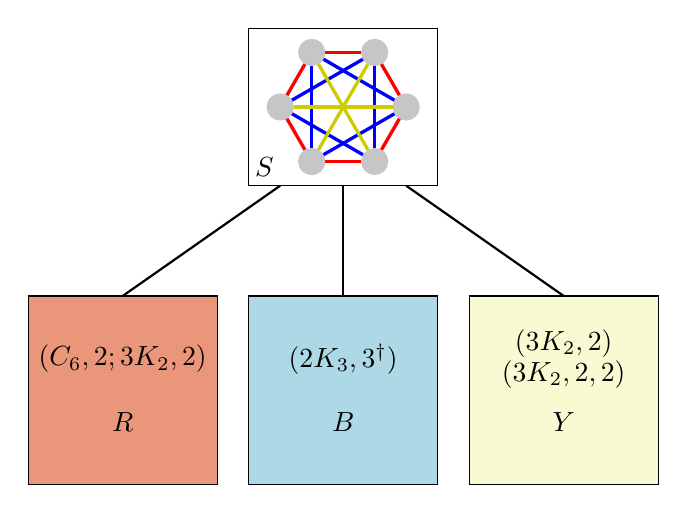
\begin{tikzpicture}[scale=0.8]
    \begin{scope}[shift = {(0,0)}]
        \draw[black] (-1.5,-1.25) rectangle ++(3,2.5);
        \node at (-1.25,-0.95) {$S$};
        \foreach \x in {0,...,5}
        {
            \node[vertex,lightgray,fill=lightgray] (p\x) at (\x*60+60:1) {};
        }
        \draw[edge,red] (p0) -- (p1);
        \draw[edge,red] (p1) -- (p2);
        \draw[edge,red] (p2) -- (p3);
        \draw[edge,red] (p3) -- (p4);
        \draw[edge,red] (p4) -- (p5);
        \draw[edge,red] (p5) -- (p0);

        \draw[edge,blue] (p0) -- (p2);
        \draw[edge,blue] (p2) -- (p4);
        \draw[edge,blue] (p4) -- (p0);
        \draw[edge,blue] (p1) -- (p3);
        \draw[edge,blue] (p3) -- (p5);
        \draw[edge,blue] (p5) -- (p1);

        \draw[edge,darkyellow] (p0) -- (p3);
        \draw[edge,darkyellow] (p1) -- (p4);
        \draw[edge,darkyellow] (p2) -- (p5);
    \end{scope}

    \begin{scope}[shift = {(-3.5,-4)}]
        \filldraw[draw=black,fill=lightred] (-1.5,-2) rectangle ++(3,3);
        \node at (0,-1) {$R$};
        \node at (0,0) {$\ipsixMatchingAndCycle$};
        \coordinate (largeRed) at (0,1) {};
    \end{scope}

    \begin{scope}[shift = {(0,-4)}]
        \filldraw[draw=black,fill=lightblue]   (-1.5,-2) rectangle ++(3,3);
        \node at (0,-1) {$B$};
        \node at (0,0) {$\ipsixTriangle$};
        \coordinate (largeBlue) at (0,1) {};
    \end{scope}

    \begin{scope}[shift = {(3.5,-4)}]
        \filldraw[draw=black,fill=lightyellow] (-1.5,-2) rectangle ++(3,3);
        \node at (0,-1) {$Y$};
        \node at (0,0.25) {$\ipsixMatching$};
        \node at (0,-0.25) {$\ipsixMatchingTwice$};
        \coordinate (largeYellow) at (0,1) {};
    \end{scope}
    \draw[edge,black,thick] (largeBlue) -- (0,-1.25);
    \draw[edge,black,thick] (largeRed) -- (-1,-1.25);
    \draw[edge,black,thick] (largeYellow) -- (1,-1.25);

\end{tikzpicture}
         \end{center}
        \subcaption{$|\ul(\inducedCC{S})| = 4$.}
        \label{restorable:6cc:monochormatic-cycle/fig}
    \end{subfigure}
    \hfill
    \begin{subfigure}[]{.4\textwidth}
        \begin{center}
            

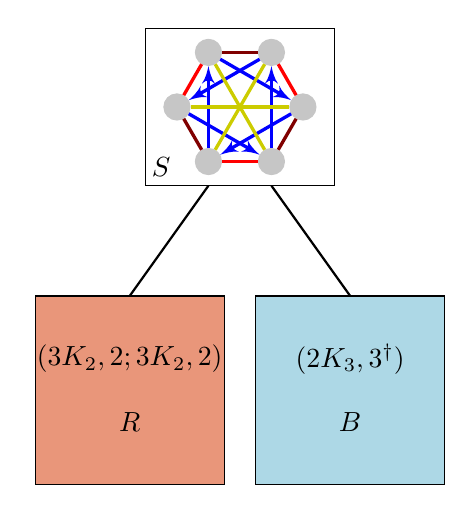
\begin{tikzpicture}[scale=0.8]

    \begin{scope}[shift = {(0,0)}]
        \draw[black] (-1.5,-1.25) rectangle ++(3,2.5);
        \node at (-1.25,-0.95) {$S$};
        \foreach \x in {0,...,5}
        {
            \node[vertex,lightgray,fill=lightgray] (p\x) at (\x*60+60:1) {};
        }
        \draw[edge,darkred] (p0) -- (p1);
        \draw[edge,red] (p1) -- (p2);
        \draw[edge,darkred] (p2) -- (p3);
        \draw[edge,red] (p3) -- (p4);
        \draw[edge,darkred] (p4) -- (p5);
        \draw[edge,red] (p5) -- (p0);

        \draw[arrow,blue] (p0) -- (p2);
        \draw[arrow,blue] (p2) -- (p4);
        \draw[arrow,blue] (p4) -- (p0);
        \draw[arrow,blue] (p1) -- (p5);
        \draw[arrow,blue] (p5) -- (p3);
        \draw[arrow,blue] (p3) -- (p1);

        \draw[edge,darkyellow] (p0) -- (p3);
        \draw[edge,darkyellow] (p1) -- (p4);
        \draw[edge,darkyellow] (p2) -- (p5);
    \end{scope}

    \begin{scope}[shift = {(-1.75,-4)}]
        \filldraw[draw=black,fill=lightred] (-1.5,-2) rectangle ++(3,3);
        \node at (0,-1) {$R$};
        \node at (0,0) {$\ipsixMatchingMatching$};
        \coordinate (largeRed) at (0,1) {};
    \end{scope}

    \begin{scope}[shift = {(1.75,-4)}]
        \filldraw[draw=black,fill=lightblue]   (-1.5,-2) rectangle ++(3,3);
        \node at (0,-1) {$B$};
        \node at (0,0) {$\ipsixTriangle$};
        \coordinate (largeBlue) at (0,1) {};
    \end{scope}

    \draw[edge,black,thick] (largeRed) -- (-0.5,-1.25);
    \draw[edge,black,thick] (largeBlue) -- (0.5,-1.25);

\end{tikzpicture}
         \end{center}
        \subcaption{$|\ul(\inducedCC{S})| = 5$.}
        \label{restorable:6cc:alternating-cycle/fig}
    \end{subfigure}
    \caption{Visualisation of the neighbor subset partition in Lemma~\ref{critical:6-cc:restorable:large-neighborhood/lem}.}
    \label{restorable:6cc/fig}
\end{figure}


\begin{lemma}
\label{critical:6-cc:restorable:large-neighborhood/lem}
    Let~$\coherentConfig$ be a critical coherent configuration and~$S \in \fibers{\coherentConfig}$ be a fiber such that~$\abs{S} = 6$, $\abs{\ul(\inducedCC{S})} > 3$, and~$\{S\}$ is not dominating.
    There exist disjoint subsets~$\mathcal{R},\mathcal{B}, \mathcal{Y}$ partitioning the neighborhood of~$S$ in~$\quotientGraph{\coherentConfig}$ with~$\mathcal{R},\mathcal{B}$ non-empty (and~$\mathcal{Y}$ possibly empty) such that
    \begin{enumerate}
        \item for all~$R \in \mathcal{R}$ the interspace~$\interspace{R}{S}$ has either interspace pattern~$\ipsixMatchingAndCycle$ or interspace pattern~$\ipsixMatchingMatching$,
        \item for all~$B \in \mathcal{B}$ the interspace~$\interspace{B}{S}$ has interspace pattern~$\ipsixTriangle$,
        \item for all~$Y \in \mathcal{Y}$ the interspace~$\interspace{Y}{S}$ has either interspace pattern~$\ipsixMatching$ or interspace pattern~$\ipsixMatchingTwice$.
    \end{enumerate}
    In particular, $\colorDeg{S} \geq 2$. (See Figure~\ref{restorable:6cc/fig})
\end{lemma}
\begin{proof}\textcolor{red}{TOPROVE 23}\end{proof}


\begin{lemma}
    \label{critical:6-cc:restorable:cycle/lem}
    Let~$\coherentConfig$ be a critical coherent configuration and~$R,S \in \fibers{\coherentConfig}$ be distinct fibers of size~$6$ such that $\cycle{12} \in \interspace{R}{S}$ and~$\{R,S\}$ is not dominating.
    There exist disjoint, non-empty subsets~$\mathcal{B}, \mathcal{Y}$ of the neighborhood of~$S$ without~$R$ in~$\quotientGraph{\coherentConfig}$ such that
    \begin{enumerate}
        \item for all~$B \in \mathcal{B}$ the interspace~$\interspace{B}{S}$ has interspace pattern~$\ipsixTriangle$ and
        \item for all~$Y \in \mathcal{Y}$ the interspace~$\interspace{Y}{S}$ has either interspace pattern~$\ipsixMatching$ or interspace pattern~$\ipsixMatchingTwice$.
    \end{enumerate}
    In particular, $\colorDeg{S} \geq 3$.
\end{lemma}
\begin{proof}\textcolor{red}{TOPROVE 24}\end{proof}


Next we deal with interspaces isomorphic to~$\interspaceFourSix \in \interspace{R}{B}$ for fibers~$R,B$ with~$|R| < |B|$.
Such an interspace has a different pattern depending on the perspective.
Interspace~$\interspace{R}{B}$ has interspace pattern~$\ipsixMatchingComplementD$, while interspace~$\interspace{B}{R}$ has interspace pattern~$\ipfourClique$.


\begin{lemma}
\label{critical:4cc-6cc/lem}
    Let~$\coherentConfig$ be critical coherent configuration, and let~$R,S \in \fibers{\coherentConfig}$ fibers such that~$\interspace{R}{S}$ has interspace pattern~$\ipsixMatchingComplementD$.
    \begin{enumerate}
        \item\label{4cc-6cc:part1}
        If~$\colorDeg{R} = 1$, then~$\{S\}$ is dominating and for all fibers~$Y$ adjacent to~$S$ in~$\quotientGraph{\coherentConfig}$ other than~$R$ the interspace~$\interspace{Y}{S}$ has either interspace pattern~$\ipsixMatching$ or interspace pattern~$\ipsixMatchingTwice$.
        \item
        If~$\interspaceFourSix \in \interspace{R}{S}$ and all fibers of~$\coherentConfig$ are small, then~$\wldim{\coherentConfig} = 2$.
    \end{enumerate}
\end{lemma}
\begin{proof}\textcolor{red}{TOPROVE 25}\end{proof}


\begin{lemma}
\label{critical:7-cc:leviFano/lem}
    If~$\coherentConfig$ is a critical coherent configuration, then there is no path~$(R,B,Y)$ in~$\quotientGraph{\coherentConfig}$ such that~$\leviFano \in \interspace{R}{B}$ and~$\leviFano \in \interspace{B}{Y}$.
\end{lemma}
\begin{proof}\textcolor{red}{TOPROVE 26}\end{proof}


\begin{lemma}
\label{restorable:two-3K2,2-ip:fully-intersecting/lem}
    Let~$\coherentConfig$ be a critical coherent configuration and~$(S,L,S')$ be a path in~$\quotientGraph{\coherentConfig}$ such that~$\interspace{L}{S}$ and~$\interspace{L}{S'}$ both have interspace pattern~$\ipsixMatching$.
    If~$|L| = 9$, $\colorDeg{L} = 2$, $|\ul(\inducedCC{L})| = 4$, and~$\equivalenceClasses{L,S}$ and~$\equivalenceClasses{L,S'}$ are fully intersecting, then~$\{L\}$ is dominating.
\end{lemma}
\begin{proof}\textcolor{red}{TOPROVE 27}\end{proof}




 


\section{Weisfeiler-Leman dimension of graphs with small fibers}
\label{wldim-small/sec}


\begin{theorem}
    \label{critical:small-cc/thm}
    Let~$\coherentConfig$ be a critical coherent configuration.
    If all fibers of~$\coherentConfig$ are small, then either
    \begin{enumerate}
        \item all fibers have the same size, or
        \item for all~$R \in \fibers{\coherentConfig}$ we have~$\abs{R} \in \{4,6\}$.
    \end{enumerate}
\end{theorem}
\begin{proof}\textcolor{red}{TOPROVE 28}\end{proof}


\begin{lemma}
\label{4-cc:cdeg-decrease/lem}
    Let~$\coherentConfig$ be a critical coherent configuration such that all fibers of~$\coherentConfig$ have size~$4$.
    A fiber~$R$ of~$\coherentConfig$ and all fibers adjacent to it in~$\quotientGraph{\coherentConfig}$ split entirely into tiny fibers in~$\coherentConfig_r$ where~$r \in R$.

    In particular, if~$\colorDeg{R} \geq 4$, then~$\wldim{\coherentConfig}=2$ or  there is a critical coherent configuration~$\coherentConfig'$ for which $\wldim{\coherentConfig} \leq  1 + \wldim{\coherentConfig_r} = 1 + \wldim{\coherentConfig'}$ with~$\abs{\vertices(\coherentConfig)} \leq \abs{\vertices(\coherentConfig')} - 20$.
\end{lemma}
\begin{proof}\textcolor{red}{TOPROVE 29}\end{proof}


The lemma essentially allows us to reduce the degree of the quotient graph. For graphs with maximum degree at most~$3$, we can make use of a bound by Fomin and H{\o}ie on the pathwidth of the graph.


\begin{theorem}[see \cite{pathwidthCubicGraphs}]
\label{tw-cubic-graph/lem}
    For every $\epsilon > 0$, there exists $n_0 \in \Nat$ such that every graph of maximum degree at most~$3$ with at at least~$n$ vertices satisfies $\treewidth(G)\leq \pathwidth(G) \leq \frac{n}{6} + \epsilon$.
\end{theorem}


We use the theorem to bound the Weisfeiler-Leman dimension for certain graphs as follows.


\begin{theorem}
\label{4-cc:cfi-wldim/thm}
    Let~$\coherentConfig$ be a critical coherent configuration on~$n$ vertices such that all fibers of~$\coherentConfig$ have size~$4$ and there is no interspace containing a constituent isomorphic to~$\cycle{8}$.
    If all fibers of~$\coherentConfig$ have at most~$3$ neighbors in~$\quotientGraph{\coherentConfig}$, then~$\wldim{\coherentConfig} \leq \frac{n}{24} + \mathcal{O}(1)$.
\end{theorem}
\begin{proof}\textcolor{red}{TOPROVE 30}\end{proof}


\begin{corollary}
\label{4-cc:wldim/cor}
    Let~$\coherentConfig$ be a critical coherent configuration on~$n$ vertices such that all fibers of~$\coherentConfig$ have size~$4$.
    Then~$\wldim{\coherentConfig} \leq \frac{n}{20} + \mathcal{O}(1)$.
\end{corollary}
\begin{proof}\textcolor{red}{TOPROVE 31}\end{proof}


\begin{lemma}
\label{5-cc:wldim/lem}
    Let~$\coherentConfig$ be a critical coherent configuration such that all fibers of~$\coherentConfig$ have size~$5$.
    Then~$\abs{\fibers{\coherentConfig}} = 1$ and~$\wldim{\coherentConfig} \leq 2$.
\end{lemma}
\begin{proof}\textcolor{red}{TOPROVE 32}\end{proof}


\begin{lemma}
\label{6-cc:wldim/lem}
    If~$\coherentConfig$ is a critical coherent configuration whose fibers each have size~$4$ or~$6$, then $\wldim{\coherentConfig} \leq \frac{n}{20}+ \mathcal{O}(1)$.
\end{lemma}
\begin{proof}\textcolor{red}{TOPROVE 33}\end{proof}


\begin{lemma}
\label{7-cc:wldim/lem}
    Let~$\coherentConfig$ be a critical coherent configuration such that all fibers of~$\coherentConfig$ have size~$7$.
    Then~$\abs{\fibers{\coherentConfig}} \leq 2$ and~$\wldim{\coherentConfig} \leq 3$.
\end{lemma}

\begin{proof}\textcolor{red}{TOPROVE 34}\end{proof}


\begin{theorem}
\label{small-cc:wldim/thm}
    Let~$\coherentConfig$ be a critical coherent configuration such that all fibers of~$\coherentConfig$ are small.
    Then~$\wldim{\coherentConfig} \leq \frac{n}{20} + \mathcal{O}(1)$.
\end{theorem}
\begin{proof}\textcolor{red}{TOPROVE 35}\end{proof}

     


\section{Limiting fiber sizes}
\label{sec:limit:fiber:sizes}


For each interspace~$\interspace{R}{B}$ we arbitrarily choose a basis relation whose degree is maximal. A \emph{non-maximal} basis relation is basis relation different than the chosen one.
Similarly for each fiber~$R$ we chose a constituent with maximal degree. A non-maximal constituent is one that is not the chosen one. Define~$\overline{\minimalDegree{B}{R}}$ to be the maximum degree among all degrees of non-maximal basis relations in~$\interspace{R}{B}$. Set~$\overline{\minimalDegree{B}{R}}=0$ if~$|\interspace{R}{B}|=1$.

Define the \emph{max-modules} of a coherent configuration to be the connected components of the graph in which the edges are formed by all non-maximal basis relations. (The max-modules are sections in the sense of~\cite{DBLP:journals/dam/Goldberg83} and colored modules in the sense of~\cite{DBLP:journals/mst/Schweitzer17}.)
It is not difficult to see that the Weisfeiler-Leman dimension of a coherent configuration is at most the maximum of~$2$ and the maximum Weisfeiler-Leman dimension of its max-modules.


\begin{lemma}[Color valence limit, (Zemlyachenko, see~\cite{DBLP:conf/fct/Babai81})]
\label{lem:bound-on-min:degree}
    Let~$\coherentConfig$ be a critical coherent configuration, let~$d \in \Nat$ be a positive integer.
    There is a set of vertices~$S$ of size at most~$\frac{2n}{d}$  so that in the components of
    $\coherentConfig_S$ we have~$\overline{\minimalDegree{B}{R}}\leq d$
     for all (not necessarily distinct) fibers~$R,B \in \fibers{\coherentConfig_S}$.
\end{lemma}
\begin{proof}\textcolor{red}{TOPROVE 36}\end{proof}


\begin{lemma}[Fiber size limit]
\label{lem:bound-on-cc-size}
    Let~$\coherentConfig$ be a critical coherent configuration, and let~$c, d \in \Nat$ be positive integers.
    There is a set~$S$ of vertices of size at most~$\frac{2n}{d} + \frac{dn}{c}$ such that for each max-module~$\overline{\coherentConfig}$ of~$\coherentConfig_S$ we have~$\abs{R} \leq c$ and~$\overline{\minimalDegree{R}{B}}\leq d$
     for all (not necessarily distinct) fibers~$R,B \in \fibers{\overline{\coherentConfig}}$.
\end{lemma}
\begin{proof}\textcolor{red}{TOPROVE 37}\end{proof}


\begin{lemma}
\label{lem:bd:tw:and:fibre:size:bd:WL}
    If all fibers of a coherent configuration~$\coherentConfig$ have size at most~$t$, then~$\wldim{\coherentConfig}\leq t\cdot \treewidth(\quotientGraph{\coherentConfig})$, where~$\treewidth(\quotientGraph{\coherentConfig})$ is the treewidth of the quotient graph.
\end{lemma}
\begin{proof}\textcolor{red}{TOPROVE 38}\end{proof}
 

\section{A potential function}
\label{sec:potential:func}


For a coherent configuration~$\coherentConfig$ let~$\parameters(\coherentConfig)$ be the triple~$(n_\ell, k_\ell,n_s)$, where~$n_\ell$ is the number of vertices in large fibers,~$k_\ell$ is the number of large fibers and~$n_s$ is the number of small fibers.

Let~$\widehat{\f} \colon \Nat^3 \longrightarrow \Nat$ be the function that assigns to the triple~$(n_\ell, k_\ell,n_s)$ the maximum Weisfeiler-Leman dimension of a coherent configuration~$\coherentConfig$ with~$\parameters(\coherentConfig)=(n_\ell, k_\ell,n_s)$.

Define the function~$\tau \colon \Nat^3 \rightarrow \Rel$ with~$(n_\ell, k_\ell, n_s) \mapsto \frac{3n_\ell + n_s - 8k_\ell}{20}$.

Note that the parameters and function~$\tau$ are additive in the sense that we can compute the parameters separately for a configuration induced by an arbitrary partition of the fibers and then add them up.

We now define~$\f$ to be the function that assigns to a coherent configuration $\coherentConfig$ the maximum Weisfeiler-Leman dimension among all coherent configurations $\coherentConfig'$ for which~$\tau(\parameters(\coherentConfig'))\leq \tau(\parameters(\coherentConfig))$. (In some sense~$f$ is a monotonization of~$\widehat{f}$.)

Using this notation, note that the choice of potential function guarantees that if~$\coherentConfig'$ is finer than~$\coherentConfig$ then~$\f(\coherentConfig')\leq \f(\coherentConfig)$.

We define $\widetilde{\f} \colon \Rel \longrightarrow \Rel$ with $r \mapsto \max \{ \f(\coherentConfig) \mid \tau (\parameters(\coherentConfig)) \leq r \}$.

Our goal in the upcoming sections will be to show that~$\wldim{\coherentConfig}\leq \tau(\parameters(\coherentConfig))+o(n)$. A key technique will be reductions that show that~$\wldim{\coherentConfig}\leq t+ \f(\tau (\parameters(\coherentConfig')))$ for some coherent configuration~$\coherentConfig'$ obtained from~$\coherentConfig$ in a controlled manner, which will give a recursive bound of the form~$\wldim{\coherentConfig}
 \leq t + \widetilde{f} (\tau(\parameters(\coherentConfig)) -t)$.     


\section{Local reductions}
\label{recursive-argement/sec}

In this section we provide local reductions,
trading progress in the potential with individualizations. This eventually allows us to restrict the structure of the coherent configuration in three ways:
First, it limits the number of neighbors a large fibers can have in the quotient graph.
Second, we eliminate certain interspace patterns. For some other interspace patterns we show that there  can be at most one small neighboring fiber attached with this pattern.
Finally we reduce the quotient graph degree of fibers of size~4 or~6.

Each reduction proceeds as follows.
We examine the local structure of neighbors of a fiber. In particular, we describe the interspace patterns and the color degree.
We individualize one or two carefully chosen vertices, take the coherent closure, and restore criticality.
Afterwards we weigh the number of individualized vertices against the progress in the terms of the potential function~$\tau$ we made due to fibers that split.

To write the proofs of this section more concisely, we introduce an auxiliary result as follows.
For triples~$(a,b,c),(a',b',c')\in \Nat^3$, we will use the notation~$(a,b,c)\preceq (a',b',c')$ to denote that~$\tau(a,b,c)\leq \tau(a',b',c')$.
Define a function~$\hfunction\colon \Rel^+\rightarrow \Rel$
by setting~$\hfunction(a)= \max\{-0.4,-3\cdot \frac{\lceil 8a\rceil }{20}\}$.










\begin{lemma}
\label{local:progress-in-large/lem}
    Let~$\coherentConfig, \coherentConfig'$ be a coherent configurations so that~$\coherentConfig$ consists of a single large fiber and~$\coherentConfig'\finer \coherentConfig$.
    Let~$R_1,\ldots,R_u$ be the fibers of~$\coherentConfig'$ and set~$\{t_i \mid i \in\{1,\ldots,u\}, |R_i|= t_i \cdot|\coherentConfig| \}$.
    Then~$\tau(\parameters(\coherentConfig'))\leq \tau(\parameters(\coherentConfig'))+\sum_{i = 1}^{u} \hfunction(t_i)+0.4$.
\end{lemma}
\begin{proof}\textcolor{red}{TOPROVE 39}\end{proof}

We should remark that while Lemma~\ref{local:progress-in-large/lem} is sufficient to calculate the progress made in~$L$ in many cases, in some other case a closer examination produces better results on the progress.
This is especially true if we know conditions on the size of~$L$ or sizes of the vertex sets into which~$L$ splits.










\begin{lemma}
    \label{lem:local-argument:3-large-neighbors}
    Let~$\coherentConfig$ be a critical coherent configuration, $R \in \fibers{\coherentConfig}$, and~$\{L_1,L_2,L_3\}$ a set of large fibers adjacent to~$R$ in~$\quotientGraph{\coherentConfig}$.
    If~$R$ is a large fiber or~$|\ul(\inducedCC{R})| \geq 3$, then~$\wldim{\coherentConfig} \leq 1 + \widetilde{\f}( \tau(\parameters(\coherentConfig)) - 1)$.
\end{lemma}
\begin{proof}\textcolor{red}{TOPROVE 40}\end{proof}


For a coherent configuration~$\coherentConfig$, we define~$\quotientGraphLarge{\coherentConfig}$ and~$\quotientGraphSmall{\coherentConfig}$ to be the subgraph of~$\quotientGraph{\coherentConfig}$ induced by the set of all large fibers and small fibers, respectively.


\begin{lemma}\label{lem:max:degree:2:means:tw:3}
    If~$\coherentConfig$ is a coherent configuration in which no large fiber has at least 3 large neighbors.
    Then the connected components of~$\quotientGraphLarge{\coherentConfig}$ have treewidth at most~$2$.
\end{lemma}

\begin{proof}\textcolor{red}{TOPROVE 41}\end{proof}










\begin{theorem}
\label{local:L-S/thm}
    Let~$\coherentConfig$ be a critical coherent configuration and suppose~$L,S \in \fibers{\coherentConfig}$ with~$L$ large and~$S$ small.
    If the set~$\{S\}$ is not dominating and the interspace~$\interspace{L}{S}$ has one of the interspace patterns~$\ipsixMatchingAndCycle$, $\ipsixMatchingMatching$, $\ipsixMatchingTwice$, $\ipsixMatchingAndComplement$, $\ipsixMatchingComplement$, $\ipsixTriangleComplement$, or $\ipsixTriangleComplementTwice$,
    then~$\wldim{\coherentConfig} \leq 1 + \widetilde{\f}( \tau(\parameters(\coherentConfig)) - 1)$.
\end{theorem}
\begin{proof}\textcolor{red}{TOPROVE 42}\end{proof}










\begin{theorem}
\label{local:S-L-S/thm}
    Let~$\coherentConfig$ be a critical coherent configuration and let~$(S,L,S')$ be a path in~$\quotientGraph{\coherentConfig}$ with~$L$ large and~$S,S'$ small.
    If~$\interspace{L}{S}$ has interspace pattern~$\ipsixMatchingComplementD$ and~$\interspace{L}{S'}$ has one of the interspace patterns~$\ipsixMatchingComplementD$, $\ipfourCycle$, $\ipsixMatching$, $\ipfourMatching$, or~$\ipsixTriangle$,
    then~$\wldim{\coherentConfig} \leq 1 + \widetilde{\f}( \tau(\parameters(\coherentConfig)) - 1.1)$.
\end{theorem}
\begin{proof}\textcolor{red}{TOPROVE 43}\end{proof}










\begin{theorem}
\label{local:S-L-S:rest/thm}
    Let~$\coherentConfig$ be a critical coherent configuration, and let~$(S,L,S')$ be a path in~$\quotientGraph{\coherentConfig}$ with~$L$ large and~$S,S'$ small.
    If~$\{S\}$ and~$\{S'\}$ are not dominating and both~$\interspace{L}{S}$ and~$\interspace{L}{S'}$ have one of the interspace patterns~$\ipfourCycle$, $\ipsixMatching$, $\ipfourMatching$, or~$\ipsixTriangle$,
    then~$\wldim{\coherentConfig} \leq 1 + \widetilde{\f}( \tau(\parameters(\coherentConfig)) - 1)$.
\end{theorem}
\begin{proof}\textcolor{red}{TOPROVE 44}\end{proof}










Given~$F \in \fibers{\coherentConfig}$, we denote the number of large (respectively small) fibers adjacent to~$F$ in~$\quotientGraph{\coherentConfig}$ by~$\colorDegLarge{F}$ (respectively~$\colorDegSmall{F}$).

\begin{lemma}
\label{local:4cc:3neighbors/lem}
    Let~$\coherentConfig$ be a critical coherent configuration, and let~$S$ be a size-$4$ fiber of~$\coherentConfig$ such that~$\clique{4} \notin\inducedCC{S}$.
    If~
    \begin{itemize}
        \item $\colorDeg{S} = 3$ and~$\colorDegLarge{S} \geq 1$ or
        \item $\colorDeg{S} \geq 4$,
    \end{itemize}
    then~$\wldim{\coherentConfig} \leq 1 + \widetilde{\f}( \tau(\parameters(\coherentConfig)) - 1)$.
\end{lemma}
\begin{proof}\textcolor{red}{TOPROVE 45}\end{proof}










\begin{lemma}
\label{local:K222-3D/lem}
    Let~$\coherentConfig$ be a critical coherent configuration, and let~$(L,S)$ be an edge in~$\quotientGraph{\coherentConfig}$ such that~$\interspace{L}{S}$ has interspace pattern~$\ipsixMatchingComplementD$.
    If~$\colorDeg{S} \geq 3$ and~$\{L,S\}$ is not dominating, then
    \begin{itemize}
        \item $\wldim{\coherentConfig} \leq 1 + \widetilde{\f}( \tau(\parameters(\coherentConfig)) - 1)$ or
        \item $\wldim{\coherentConfig} \leq 2 + \widetilde{\f}( \tau(\parameters(\coherentConfig)) - 2.1)$
    \end{itemize}
\end{lemma}
\begin{proof}\textcolor{red}{TOPROVE 46}\end{proof}




\begin{lemma}
\label{local:alternating-6cycle/lem}
    Let~$\coherentConfig$ be a critical coherent configuration, and let~$(L,S,S')$ be a path in~$\quotientGraph{\coherentConfig}$ such that interspace~$\interspace{L}{S}$ has interspace pattern~$\ipsixMatchingComplementD$ and interspace~$\interspace{S}{S'}$ has interspace pattern~$\ipsixMatchingMatching$.
    If~$\{L,S\}$ is not dominating, then
    \begin{itemize}
        \item $\wldim{\coherentConfig} \leq 1 + \widetilde{\f}( \tau(\parameters(\coherentConfig)) - 1.05)$ or
        \item $\wldim{\coherentConfig} \leq 2 + \widetilde{\f}( \tau(\parameters(\coherentConfig)) - 2)$.
    \end{itemize}
\end{lemma}
\begin{proof}\textcolor{red}{TOPROVE 47}\end{proof}










\begin{lemma}
\label{local:6cc:3neighbors/lem}
    Let~$\coherentConfig$ be a critical coherent configuration, and let~$S$ be a size~$6$ fiber of~$\coherentConfig$  such that~$\clique{6} \notin\inducedCC{S}$.
    If~$\colorDeg{S} \geq 3$, then~$\wldim{\coherentConfig} \leq 1 + \widetilde{\f}( \tau(\parameters(\coherentConfig)) - 1  )$.
\end{lemma}
\begin{proof}\textcolor{red}{TOPROVE 48}\end{proof}

     


\section{The structure of reduced coherent configurations}
\label{structure-reduced-cc/sec}

Let~$\coherentConfig$ be a coherent configuration.
We call a small fiber~$S$~\emph{relevant} if~$|S| \in \{4,6\}$ and~$|\ul(\inducedCC{S})| > 2$, and~\emph{irrelevant} otherwise.
For a fiber~$R$ of~$\coherentConfig$, we define~$\colorDegRelevantSmall{R}$ to be number of relevant small fibers adjacent to~$R$ in~$\quotientGraph{\coherentConfig}$.


\begin{lemma}
\label{irrelevant-small-fibers/lem}
    Let~$\coherentConfig$ be a critical coherent configuration.
    If~$S$ is an irrelevant small fiber of~$\coherentConfig$,
    then~$\colorDegSmall{S} \leq 1$ and the set of fibers adjacent to~$S$ in~$\quotientGraph{\coherentConfig}$ induces a clique in~$\quotientGraph{\coherentConfig}$.

    Furthermore, if~$\colorDegLarge{S} \geq 1$, then~$S$ is not adjacent to an relevant in~$\quotientGraph{\coherentConfig}$.
\end{lemma}
\begin{proof}\textcolor{red}{TOPROVE 49}\end{proof}


\begin{lemma}
\label{dominating:wldim/lem}
    Let~$\coherentConfig$ be a critical coherent configuration and there is~$t \in \Nat$ such that all fibers of~$\coherentConfig$ have size at most~$t$.
    If there is a set of fibers~$\mathcal{R}$ which is dominating and there are at most~$u \in \Nat$ large fibers adjacent to a fiber of~$\mathcal{R}$, then~$\wldim{\coherentConfig} \leq 2 + \sum_{R \in \mathcal{R}} |R| + u \cdot t$.
\end{lemma}
\begin{proof}\textcolor{red}{TOPROVE 50}\end{proof}


\begin{definition}
\label{new:global-argument:assumption}
    For~$t\in \Nat$, we call a coherent configuration~$\coherentConfig$ \emph{$t$-reduced}, if it satisfies all of the following properties.
    \begin{enumerate}
        \item \label{new:global-argument:assumption:critical}
        $\coherentConfig$ is critical.
        \item \label{new:global-argument:assumption:limited-fiber-size}
        Every fiber~$R$ has at most~$t$ vertices, i.e.,~$|R|\leq t$.
        \item \label{new:global-argument:assumption:large-colorDeg}
        All large fibers~$L$ have at most two large neighbors, that is~$\colorDegLarge{L} \leq 2$.
        \item \label{new:global-argument:assumption:large-one-relevent}
        A large fiber has at most one relevant small neighbor, that is~$\colorDegRelevantSmall{L} \leq 1$.
        \item \label{new:global-argument:assumption:relevant-2-neighbors}
        If a relevant small fiber~$S$ has a large neighbor (i.e., if~$\colorDegLarge{S}\geq 1$), then~$|\ul(\inducedCC{S})| = 3$ and its color degree is at most 2 (i.e., $\colorDeg{S}\leq 2$).
        \item \label{new:global-argument:assumption:relevant-3-neighbors}
        For every~$s\in S$ in a relevant small fiber~$S$ with three small neighbors (i.e.,~$\colorDegSmall{S}\geq 3$), we have that~$S$ is discrete in~$\coherentConfig_s$.
    \end{enumerate}
\end{definition}




\begin{lemma}\label{lem:properties:or:t:reduced}
    Let~$\coherentConfig$ be a critical coherent configuration whose largest fibers have size~$t$.
    Then
    \begin{itemize}
        \item $\wldim{\coherentConfig} \leq z + \widetilde{\f}( \tau(\parameters(\coherentConfig)) - z)$ for positive integer~$z$,
        \item $\wldim{\coherentConfig} \leq 10 + 2\cdot t$, or
        \item $\coherentConfig$ is $t$-reduced (i.e., satisfies Definition~\ref{new:global-argument:assumption}).
    \end{itemize}
\end{lemma}
\begin{proof}\textcolor{red}{TOPROVE 51}\end{proof}
     

\section{A global argument}
\label{global-argument/sec}

\begin{lemma}
\label{global-argument:LSL/lem}
    Let~$\coherentConfig$ be a critical coherent configuration that is $t$-reduced (Definition~\ref{new:global-argument:assumption}), and let~$(L,S,L')$ be an induced path in~$\quotientGraph{\coherentConfig}$ such that~$L, L'$ are large and $S$ is small and relevant.
    There are~$s_{1},\dots,s_{|S|/2 -1} \in S$ such that either vertex sets~$L \cup S$ and~$L'$ or the vertex sets~$L$ and~$L' \cup S$ are homogeneously connected in~$(\coherentConfig[L \cup S \cup L'])_{s_1,\dots,s_{x-1}}$.
    Furthermore~$L$ or~$L'$ has at least size~$9$ if~$|S| = 6$.
\end{lemma}
\begin{proof}\textcolor{red}{TOPROVE 52}\end{proof}



\begin{lemma}
\label{global-argument:LSSL/lem}
    Let~$\coherentConfig$ be a critical coherent configuration that is $t$-reduced (Definition~\ref{new:global-argument:assumption}), and let~$(L_0 ,S_0 ,S_1, L_1)$ be an induced path in~$\quotientGraph{\coherentConfig}$ such that~$L_0, L_1$ are large and~$S_0, S_1$ are small and relevant.
    There are~$s_{1},\dots,s_{|S_0|/2 -1} \in S_0$ such that vertex sets~$L_0 \cup S_0$ and~$L_1 \cup S_1$ are homogeneously connected in~$(\coherentConfig[L_0 \cup S_0 \cup S_1 \cup L_1])_{s_1,\dots,s_{|S_0|/2-1}}$.
\end{lemma}
\begin{proof}\textcolor{red}{TOPROVE 53}\end{proof}


\begin{lemma}
\label{lem:the:newest:global-argument}
    Let~$\coherentConfig$ be a ~$t$-reduced critical coherent configuration with parameters~$Par(\coherentConfig)=(n_\ell, k_\ell,n_s)$.
    There is a set~$M$ of size~$q\leq k_\ell$ such that each connected component of~$\quotientGraph{\coherentConfig_M}$
    \begin{itemize}
        \item induces a configuration of Weisfeiler-Leman dimension at most~$3t$ or
        \item has only small fibers and order at most~$n_s - r_1 \cdot 3-r_2\cdot 4$, where~$r_1\cdot 8.5 +r_2\cdot 8\leq n_\ell$.
    \end{itemize}
\end{lemma}
\begin{proof}\textcolor{red}{TOPROVE 54}\end{proof}


\begin{corollary}
\label{cor:of:main:global}
    Let~$\coherentConfig$ be a critical coherent configuration that is~$t$-reduced. Suppose~$Par(\coherentConfig)=(n_\ell, k_\ell,n_s)$ are the parameters of~$\coherentConfig$.

    Then~$\wldim{\coherentConfig}\leq \frac{2}{20} n_\ell + \frac{1}{20}n_s+3t\leq \tau(n_\ell, k_\ell,n_s) + 3t$.
\end{corollary}
\begin{proof}\textcolor{red}{TOPROVE 55}\end{proof}

     


\section{Proof of the main theorem}
\label{sec:proof:of:main:thm}


\begin{theorem}
    Let~$\coherentConfig$ be a coherent configuration in which every fiber has size at most~$t$ with parameters $Par(\coherentConfig)=(n_\ell, k_\ell,n_s)$,  then~$\wldim{\coherentConfig}\leq \tau(n_\ell, k_\ell,n_s)+3\cdot t+6$.
\end{theorem}
\begin{proof}\textcolor{red}{TOPROVE 56}\end{proof}

\begin{theorem}
    Let~$\coherentConfig$ be a coherent configuration on~$n$ vertices then~$\wldim{\coherentConfig}\leq 3/20 n + o(n)$.
\end{theorem}
\begin{proof}\textcolor{red}{TOPROVE 57}\end{proof}
     
\section{Lower bound}
\label{sec:lower:bound}


In this section we assemble several known results to obtain an improved lower bound for the maximum Weisfeiler-Leman dimension of graphs in terms of their order.


\begin{theorem}
    A random cubic graph asymptotically almost surely has a treewidth of at least~$ 0.042011151 \cdot n$.
\end{theorem}
\begin{proof}\textcolor{red}{TOPROVE 58}\end{proof}


It is well known that cubic graphs of high treewidth yield graphs with high Weisfeiler-Leman dimension via the CFI-construction.
Specifically, we have the following relation.


\begin{theorem}[Consequence of {\cite[Theorem 3]{DBLP:conf/csl/DawarR07}}]
    For a graph~$G$, the CFI-graph~$CFI(G)$ with base graph~$G$ satisfies~$\wldim{G}\geq \treewidth(G)$.
\end{theorem}


We remark that there are two versions of the CFI-constructions used in the literature. One where each vertex is replaced by a gadget of order 10 and one where each vertex is replaced by a gadget of order 4. (See~\cite{DBLP:conf/icalp/Furer01,DBLP:conf/esa/NeuenS17,tuprints24244} for more information.)
These versions are very similar and the theorem, as well as many other theorems, hold for either of them.
The difference between the constructions is that the former produces CFI-graphs of order~$10 |G|$, while the latter produces graphs of order~$4|G|$. In the terminology of our current paper, the first version produces coherent configurations with fibers of size 2, so a non-critical configuration. Removal of the tiny fibers yields the other construction.


The two theorems combine as follows.


\begin{corollary}
    The maximum Weisfeiler-Leman dimension for cubic graphs of order~$n$ is at least~$0.0105027 \cdot  n -o(n)$.
\end{corollary}


In the light of our discussions in Section~\ref{small-cc/sec} we remark that, due to the nature of the CFI-construction, the statement is also true for graphs of color class size 4.     \bibliography{bib/bound-wldim}

\end{document}